\documentclass[a4paper]{article}

\def\nbook {Introduction to Electrodynamics \\ Fourth Edition}
\def\nbookshort {Griffiths Electrodynamics}

% Shared preamble. The fallback lets the document build whether the working
% directory is its own folder or the project root.
\IfFileExists{headerintroelectrodynamics.tex}{%%%%%%%%%%%%%%%%%%%%
% AUTHOR AND HEADER
% define \nbook
%%%%%%%%%%%%%%%%%%%%

\makeatletter
\ifx \nauthor\undefined
	\def\nauthor{David A. Lee}
\else
\fi

\author{\nbook \\ \small David J. Griffiths \\ \small Solutions by \nauthor}
\date{}

%%%%%%%%%%%%%%%%%%%%
% PACKAGES
%%%%%%%%%%%%%%%%%%%%

\usepackage{alltt} 
\usepackage{amsfonts}
\usepackage{amsmath}
\usepackage{amssymb}
\usepackage{amsthm}
\usepackage{bm}
\usepackage{booktabs}
\usepackage{caption}
\usepackage{centernot}
\usepackage{enumitem}
\usepackage{fancyhdr}
\usepackage[T1]{fontenc}
\usepackage{graphicx}
% The documents sit one level below the project root, where the ScriptR/BoldR
% symbol PDFs and the chapN/ figure folders live. Listing both "./" and "../"
% lets those be referenced the same way regardless of where the build runs.
\graphicspath{{./}{../}}
\usepackage{mathdots}
\usepackage{mathtools}
% \usepackage{microtype}
\usepackage{multirow}
\usepackage{pdflscape}
\usepackage{pgfplots}
\pgfplotsset{compat=1.18}
\usepackage{siunitx}
\usepackage{slashed}
\usepackage{tabularx}
\usepackage{tikz}
\usepackage{titletoc}
\usepackage{tkz-euclide}
\usepackage[normalem]{ulem}
\usepackage{url}
\usepackage[all]{xy}
\usepackage{imakeidx}

% fonts
% use \textsf for the sans family (problem titles, section headings)
% Latin Modern Sans, not CM Bright: cmbr under T1 has no Type 1 outlines, so it
% renders as Type 3 bitmaps, which TeXpresso's viewer cannot draw at all.
\renewcommand{\sfdefault}{lmss} % keeps default font Computer Modern Roman

% makeindex for table of contents
\makeindex[intoc, title=Index]
\indexsetup{othercode={\lhead{ Index }}}

% table of contents remove numbering
\usepackage{tocloft} % for coloring subsections -- note that sections have standard document hyperlink coloring, i.e. color = doc
\setcounter{secnumdepth}{0} % remove numbering
\renewcommand{\cftsubsecfont}{\hypersetup{linkcolor=subsect!90}} % subsection coloring
\renewcommand{\cftsubsubsecfont}{\hypersetup{linkcolor=subsubsect!90}} % subsubsection coloring
\renewcommand{\contentsname}{\textsf{Table of Contents}}

% pagestyle
\pagestyle{fancyplain}

% header
\lhead{	\nouppercase{\leftmark} }
\ifx \nextra \undefined
  \rhead{
    \ifnum\thepage=1
    \else
      \nbookshort \  | \nauthor
    \fi}
\else
  \rhead{
    \ifnum\thepage=1
    \else
      \nbookshort (\nextra)
    \fi}
\fi

% proof environment
\newcommand{\prooffont}{\scshape}
\usepackage{xpatch}
\tracingpatches
\xpatchcmd{\proof}{\itshape}{\prooffont}{}{}

% Griffiths Physics Script-R
\def\rcurs{{\mbox{$\resizebox{!}{.08in}{
\includegraphics{../ScriptR_cropped}}$}}}
\def\brcurs{{\mbox{$\resizebox{!}{.08in}{
\includegraphics{../BoldR_cropped}}$}}}
\def\hrcurs{{\mbox{$\hat \brcurs$}}}

% Python environment (for typesetting Python code)

% Default fixed font does not support bold face
\DeclareFixedFont{\ttb}{T1}{txtt}{bx}{n}{8} % for bold
\DeclareFixedFont{\ttm}{T1}{txtt}{m}{n}{8}  % for normal

% Custom colors
\usepackage{color}
\definecolor{deepblue}{rgb}{0,0,0.5}
\definecolor{deepred}{rgb}{0.6,0,0}
\definecolor{deepgreen}{rgb}{0,0.5,0}

\usepackage{listings}

% Python style for highlighting
\newcommand\pythonstyle{\lstset{
language=Python,
basicstyle=\ttm,
morekeywords={self},              % Add keywords here
keywordstyle=\ttb\color{deepblue},
emph={MyClass,__init__},          % Custom highlighting
emphstyle=\ttb\color{deepred},    % Custom highlighting style
stringstyle=\color{deepgreen},
frame=tb,                         % Any extra options here
showstringspaces=false
}}


% Python environment
\lstnewenvironment{python}[1][]
{
\pythonstyle
\lstset{#1}
}
{}

% Python for external files
\newcommand\pythonexternal[2][]{{
\pythonstyle
\lstinputlisting[#1]{#2}}}

% Python for inline
\newcommand\pythoninline[1]{{\pythonstyle\lstinline!#1!}}

%%%%%%%%%%%%%
% FUNCTIONS %
%%%%%%%%%%%%%

\DeclarePairedDelimiter\abs{\lvert}{\rvert}%
\DeclarePairedDelimiter\norm{\lVert}{\rVert}%

%%%%%%%%%%%%%%%%%%%%
% DOCUMENT GEOMETRY
%%%%%%%%%%%%%%%%%%%%

\ifx \ntrim \undefined
\else
  \usepackage{geometry}
  \geometry{
	  papersize={379pt, 699pt},
	  textwidth=345pt,
	  left=17pt,
	  top=54pt,
	  right=17pt,
  }
\fi

% maketitle statement
\title{}
\ifx \nisofficial \undefined
\let\@real@maketitle\maketitle
\renewcommand{\maketitle}{\@real@maketitle\begin{center}\begin{minipage}[c]{0.9\textwidth}\centering\footnotesize All errors, typographical and substantive, and other offenses, are entirely my own.\end{minipage}\end{center}}
\else
\fi

%%%%%%%%%%%%%%%%%%%%
% THEOREMS
%%%%%%%%%%%%%%%%%%%%

%\theoremstyle{definition}
\newtheorem*{axiom}{Axiom}
\newtheorem*{claim}{Claim}
\newtheorem*{conjecture}{Conjecture}
\newtheorem*{cor}{Corollary}
%\newtheorem*{dfn}{Definition}
\newtheorem*{eg}{Example}
\newtheorem*{ex}{Exercise}
%\newtheorem*{lemma}{Lemma}
\newtheorem*{prop}{Proposition}
%\newtheorem*{thm}{Theorem}
\newtheorem*{remark}{Remark}
\newtheorem*{warning}{Warning}

%%%%%%%%%%%%%%%%%%%%
% FORMATTING AESTHETICS
%%%%%%%%%%%%%%%%%%%%

% itemize bullets
\renewcommand{\labelitemi}{-}
\renewcommand{\labelitemii}{$\circ$}
\renewcommand{\labelenumi}{(\roman{*})}

% new page section
%\let\stdsection\section
%\renewcommand\section{\newpage\stdsection}

% new page subsection
%\let\stdsubsection\subsection
%\renewcommand\subsection{\newpage\stdsubsection}

%%%%%%%%%%%%%%%%%%%%
% \mathbb commands
%%%%%%%%%%%%%%%%%%%%

\newcommand{\C}{\mathbb{C}}
\newcommand{\N}{\mathbb{N}}
\newcommand{\Q}{\mathbb{Q}}
\newcommand{\R}{\mathbb{R}}
\newcommand{\Z}{\mathbb{Z}}

%%%%%%%%%%%%%%%%%%%%
% Complex Numbers
%%%%%%%%%%%%%%%%%%%%

\DeclareMathOperator{\Real}{Re}
\DeclareMathOperator{\Imag}{Im}

%%%%%%%%%%%%%%%%%%%%
% Probability Operators
%%%%%%%%%%%%%%%%%%%%

\DeclareMathOperator{\Bernoulli}{Bernoulli}
\DeclareMathOperator{\betaD}{Beta}
\DeclareMathOperator{\bias}{\textsf{bias}}
\DeclareMathOperator{\binomial}{Binomial}
\DeclareMathOperator{\corr}{Corr}
\DeclareMathOperator{\cov}{\textsf{Cov}}
\DeclareMathOperator{\Exp}{Exp}
\DeclareMathOperator{\gammaD}{Gamma}
\DeclareMathOperator{\mse}{\textsf{MSE}}
\DeclareMathOperator{\multinomial}{Multinomial}
\DeclareMathOperator{\Poisson}{Poisson}
\DeclareMathOperator{\sd}{sd}
\DeclareMathOperator{\se}{\textsf{se}}
\DeclareMathOperator{\Uniform}{Uniform}
\newcommand{\Prob}{\mathbb{P}}
\newcommand{\var}{\mathbb{V}}
\newcommand{\E}{\mathbb{E}}

%%%%%%%%%%%%%%%%%%%%
% TCOLORBOX CODE FROM SeniorMars
%%%%%%%%%%%%%%%%%%%%

%\usepackage[varbb]{newpxmath} changes math font to newpxmath
\usepackage{xfrac}
\usepackage[makeroom]{cancel}
\usepackage{mathtools}
\usepackage{bookmark}
\usepackage{enumitem}
\usepackage{hyperref}
\usepackage{theoremref}
\hypersetup{
	pdftitle={Assignment},
	colorlinks=true, linkcolor=doc!90,
	bookmarksnumbered=true,
	bookmarksopen=true
}
\usepackage[most,many,breakable]{tcolorbox}
\usepackage{xcolor}
\usepackage{varwidth}
\usepackage{varwidth}
\usepackage{etoolbox}
%\usepackage{authblk}
\usepackage{nameref}
\usepackage{multicol,array}
\usepackage{tikz-cd}
\usepackage[ruled,vlined,linesnumbered]{algorithm2e}
\usepackage{comment} % enables the use of multi-line comments (\ifx \fi)
\usepackage{import}
\usepackage{xifthen}
\usepackage{pdfpages}
\usepackage{transparent}

\newcommand\mycommfont[1]{\footnotesize\ttfamily\textcolor{blue}{#1}}
\SetCommentSty{mycommfont}
\newcommand{\incfig}[1]{%
    \def\svgwidth{\columnwidth}
    \import{./figures/}{#1.pdf_tex}
}

\usepackage{tikzsymbols}

% colors -- change them as you may!

\definecolor{myg}{RGB}{56, 140, 70}
\definecolor{myb}{RGB}{45, 111, 177}
\definecolor{myr}{RGB}{199, 68, 64}
\definecolor{mytheorembg}{HTML}{F2F2F9}
\definecolor{mytheoremfr}{HTML}{00007B}
\definecolor{mylenmabg}{HTML}{FFFAF8}
\definecolor{mylenmafr}{HTML}{983b0f}
\definecolor{mypropbg}{HTML}{f2fbfc}
\definecolor{mypropfr}{HTML}{191971}
\definecolor{myexamplebg}{HTML}{F2FBF8}
\definecolor{myexamplefr}{HTML}{88D6D1}
\definecolor{myexampleti}{HTML}{2A7F7F}
\definecolor{mydefinitbg}{HTML}{E5E5FF}
\definecolor{mydefinitfr}{HTML}{3F3FA3}
\definecolor{notesgreen}{RGB}{0,162,0}
\definecolor{myp}{RGB}{197, 92, 212}
\definecolor{mygr}{HTML}{880808}
\definecolor{myred}{RGB}{127,0,0}
\definecolor{myyellow}{RGB}{169,121,69}
\definecolor{myexercisebg}{HTML}{F2FBF8}
\definecolor{myexercisefg}{HTML}{88D6D1}
\definecolor{doc}{RGB}{0,0,255}
\definecolor{subsect}{RGB}{255,0,0}
\definecolor{subsubsect}{RGB}{128,0,255}
\definecolor{question}{HTML}{3FB69E}

%================================
% THEOREM BOX
%================================

%\providecommand\theoremnumber{}
\tcbuselibrary{theorems,skins,hooks}
\newtcbtheorem{Theorem}{Theorem}
{%
	enhanced,
	breakable,
	colback = mytheorembg,
	frame hidden,
	boxrule = 0sp,
	borderline west = {2pt}{0pt}{mytheoremfr},
	sharp corners,
	detach title,
	before upper = \tcbtitle\par\smallskip,
	coltitle = mytheoremfr,
	fonttitle = \bfseries\sffamily,
	description font = \mdseries,
	separator sign none,
	segmentation style={solid, mytheoremfr},
}
{th}


%================================
% Question BOX
%================================

\makeatletter
\newtcbtheorem{question}{Problem}{enhanced,
	breakable,
	colback=white,
	colframe=question,
	attach boxed title to top left={yshift*=-\tcboxedtitleheight},
	fonttitle=\bfseries\sffamily,
	title={#2},
	boxed title size=title,
	boxed title style={%
			sharp corners,
			rounded corners=northwest,
			colback=tcbcolframe,
			boxrule=0pt,
		},
	underlay boxed title={%
			\path[fill=tcbcolframe] (title.south west)--(title.south east)
			to[out=0, in=180] ([xshift=5mm]title.east)--
			(title.center-|frame.east)
			[rounded corners=\kvtcb@arc] |-
			(frame.north) -| cycle;
		},
	#1
}{def}
\makeatother

%================================
% PROPERTIES BOX
%================================

\tcbuselibrary{theorems,skins,hooks}
\newtcbtheorem{Property}{Property}
{%
	enhanced,
	breakable,
	colback = mytheorembg,
	frame hidden,
	boxrule = 0sp,
	borderline west = {2pt}{0pt}{mytheoremfr},
	sharp corners,
	detach title,
	before upper = \tcbtitle\par\smallskip,
	coltitle = mytheoremfr,
	fonttitle = \bfseries\sffamily,
	description font = \mdseries,
	separator sign none,
	segmentation style={solid, mytheoremfr},
}
{th}

%================================
% LEMMA
%================================

\tcbuselibrary{theorems,skins,hooks}
\newtcbtheorem[number within=section]{Lemma}{Lemma}
{%
	enhanced,
	breakable,
	colback = mylenmabg,
	frame hidden,
	boxrule = 0sp,
	borderline west = {2pt}{0pt}{mylenmafr},
	sharp corners,
	detach title,
	before upper = \tcbtitle\par\smallskip,
	coltitle = mylenmafr,
	fonttitle = \bfseries\sffamily,
	description font = \mdseries,
	separator sign none,
	segmentation style={solid, mylenmafr},
}
{th}


% Commands for special boxes
\newcommand{\thm}[2]{\begin{Theorem*}{#1}{}#2\end{Theorem*}}
\newcommand{\qs}[2]{\begin{question*}{#1}{}#2\end{question*}}
\newcommand{\prp}[2]{\begin{Property*}{#1}{}#2\end{Property*}}
\newcommand{\lemma}[2]{\begin{Lemma*}{#1}{}#2\end{Lemma*}}


%%%%%%%%%%%%%%%%%%%%
% SHARED DOCUMENT SETTINGS
%%%%%%%%%%%%%%%%%%%%
% Moved here from the chapter document's preamble so that every document
% (chapters and the merged manual) picks up the same settings from one place.

\hfuzz=125pt      % ignore overfull boxes up to 5pt
\hbadness=10000   % suppress underfull warnings

\usetikzlibrary{arrows.meta, calc, decorations.markings, backgrounds}
\usepackage{tikz-3dplot}
\usepackage{float}
\usepackage{esint}
}{%%%%%%%%%%%%%%%%%%%%
% AUTHOR AND HEADER
% define \nbook
%%%%%%%%%%%%%%%%%%%%

\makeatletter
\ifx \nauthor\undefined
	\def\nauthor{David A. Lee}
\else
\fi

\author{\nbook \\ \small David J. Griffiths \\ \small Solutions by \nauthor}
\date{}

%%%%%%%%%%%%%%%%%%%%
% PACKAGES
%%%%%%%%%%%%%%%%%%%%

\usepackage{alltt} 
\usepackage{amsfonts}
\usepackage{amsmath}
\usepackage{amssymb}
\usepackage{amsthm}
\usepackage{bm}
\usepackage{booktabs}
\usepackage{caption}
\usepackage{centernot}
\usepackage{enumitem}
\usepackage{fancyhdr}
\usepackage[T1]{fontenc}
\usepackage{graphicx}
% The documents sit one level below the project root, where the ScriptR/BoldR
% symbol PDFs and the chapN/ figure folders live. Listing both "./" and "../"
% lets those be referenced the same way regardless of where the build runs.
\graphicspath{{./}{../}}
\usepackage{mathdots}
\usepackage{mathtools}
% \usepackage{microtype}
\usepackage{multirow}
\usepackage{pdflscape}
\usepackage{pgfplots}
\pgfplotsset{compat=1.18}
\usepackage{siunitx}
\usepackage{slashed}
\usepackage{tabularx}
\usepackage{tikz}
\usepackage{titletoc}
\usepackage{tkz-euclide}
\usepackage[normalem]{ulem}
\usepackage{url}
\usepackage[all]{xy}
\usepackage{imakeidx}

% fonts
% use \textsf for the sans family (problem titles, section headings)
% Latin Modern Sans, not CM Bright: cmbr under T1 has no Type 1 outlines, so it
% renders as Type 3 bitmaps, which TeXpresso's viewer cannot draw at all.
\renewcommand{\sfdefault}{lmss} % keeps default font Computer Modern Roman

% makeindex for table of contents
\makeindex[intoc, title=Index]
\indexsetup{othercode={\lhead{ Index }}}

% table of contents remove numbering
\usepackage{tocloft} % for coloring subsections -- note that sections have standard document hyperlink coloring, i.e. color = doc
\setcounter{secnumdepth}{0} % remove numbering
\renewcommand{\cftsubsecfont}{\hypersetup{linkcolor=subsect!90}} % subsection coloring
\renewcommand{\cftsubsubsecfont}{\hypersetup{linkcolor=subsubsect!90}} % subsubsection coloring
\renewcommand{\contentsname}{\textsf{Table of Contents}}

% pagestyle
\pagestyle{fancyplain}

% header
\lhead{	\nouppercase{\leftmark} }
\ifx \nextra \undefined
  \rhead{
    \ifnum\thepage=1
    \else
      \nbookshort \  | \nauthor
    \fi}
\else
  \rhead{
    \ifnum\thepage=1
    \else
      \nbookshort (\nextra)
    \fi}
\fi

% proof environment
\newcommand{\prooffont}{\scshape}
\usepackage{xpatch}
\tracingpatches
\xpatchcmd{\proof}{\itshape}{\prooffont}{}{}

% Griffiths Physics Script-R
\def\rcurs{{\mbox{$\resizebox{!}{.08in}{
\includegraphics{../ScriptR_cropped}}$}}}
\def\brcurs{{\mbox{$\resizebox{!}{.08in}{
\includegraphics{../BoldR_cropped}}$}}}
\def\hrcurs{{\mbox{$\hat \brcurs$}}}

% Python environment (for typesetting Python code)

% Default fixed font does not support bold face
\DeclareFixedFont{\ttb}{T1}{txtt}{bx}{n}{8} % for bold
\DeclareFixedFont{\ttm}{T1}{txtt}{m}{n}{8}  % for normal

% Custom colors
\usepackage{color}
\definecolor{deepblue}{rgb}{0,0,0.5}
\definecolor{deepred}{rgb}{0.6,0,0}
\definecolor{deepgreen}{rgb}{0,0.5,0}

\usepackage{listings}

% Python style for highlighting
\newcommand\pythonstyle{\lstset{
language=Python,
basicstyle=\ttm,
morekeywords={self},              % Add keywords here
keywordstyle=\ttb\color{deepblue},
emph={MyClass,__init__},          % Custom highlighting
emphstyle=\ttb\color{deepred},    % Custom highlighting style
stringstyle=\color{deepgreen},
frame=tb,                         % Any extra options here
showstringspaces=false
}}


% Python environment
\lstnewenvironment{python}[1][]
{
\pythonstyle
\lstset{#1}
}
{}

% Python for external files
\newcommand\pythonexternal[2][]{{
\pythonstyle
\lstinputlisting[#1]{#2}}}

% Python for inline
\newcommand\pythoninline[1]{{\pythonstyle\lstinline!#1!}}

%%%%%%%%%%%%%
% FUNCTIONS %
%%%%%%%%%%%%%

\DeclarePairedDelimiter\abs{\lvert}{\rvert}%
\DeclarePairedDelimiter\norm{\lVert}{\rVert}%

%%%%%%%%%%%%%%%%%%%%
% DOCUMENT GEOMETRY
%%%%%%%%%%%%%%%%%%%%

\ifx \ntrim \undefined
\else
  \usepackage{geometry}
  \geometry{
	  papersize={379pt, 699pt},
	  textwidth=345pt,
	  left=17pt,
	  top=54pt,
	  right=17pt,
  }
\fi

% maketitle statement
\title{}
\ifx \nisofficial \undefined
\let\@real@maketitle\maketitle
\renewcommand{\maketitle}{\@real@maketitle\begin{center}\begin{minipage}[c]{0.9\textwidth}\centering\footnotesize All errors, typographical and substantive, and other offenses, are entirely my own.\end{minipage}\end{center}}
\else
\fi

%%%%%%%%%%%%%%%%%%%%
% THEOREMS
%%%%%%%%%%%%%%%%%%%%

%\theoremstyle{definition}
\newtheorem*{axiom}{Axiom}
\newtheorem*{claim}{Claim}
\newtheorem*{conjecture}{Conjecture}
\newtheorem*{cor}{Corollary}
%\newtheorem*{dfn}{Definition}
\newtheorem*{eg}{Example}
\newtheorem*{ex}{Exercise}
%\newtheorem*{lemma}{Lemma}
\newtheorem*{prop}{Proposition}
%\newtheorem*{thm}{Theorem}
\newtheorem*{remark}{Remark}
\newtheorem*{warning}{Warning}

%%%%%%%%%%%%%%%%%%%%
% FORMATTING AESTHETICS
%%%%%%%%%%%%%%%%%%%%

% itemize bullets
\renewcommand{\labelitemi}{-}
\renewcommand{\labelitemii}{$\circ$}
\renewcommand{\labelenumi}{(\roman{*})}

% new page section
%\let\stdsection\section
%\renewcommand\section{\newpage\stdsection}

% new page subsection
%\let\stdsubsection\subsection
%\renewcommand\subsection{\newpage\stdsubsection}

%%%%%%%%%%%%%%%%%%%%
% \mathbb commands
%%%%%%%%%%%%%%%%%%%%

\newcommand{\C}{\mathbb{C}}
\newcommand{\N}{\mathbb{N}}
\newcommand{\Q}{\mathbb{Q}}
\newcommand{\R}{\mathbb{R}}
\newcommand{\Z}{\mathbb{Z}}

%%%%%%%%%%%%%%%%%%%%
% Complex Numbers
%%%%%%%%%%%%%%%%%%%%

\DeclareMathOperator{\Real}{Re}
\DeclareMathOperator{\Imag}{Im}

%%%%%%%%%%%%%%%%%%%%
% Probability Operators
%%%%%%%%%%%%%%%%%%%%

\DeclareMathOperator{\Bernoulli}{Bernoulli}
\DeclareMathOperator{\betaD}{Beta}
\DeclareMathOperator{\bias}{\textsf{bias}}
\DeclareMathOperator{\binomial}{Binomial}
\DeclareMathOperator{\corr}{Corr}
\DeclareMathOperator{\cov}{\textsf{Cov}}
\DeclareMathOperator{\Exp}{Exp}
\DeclareMathOperator{\gammaD}{Gamma}
\DeclareMathOperator{\mse}{\textsf{MSE}}
\DeclareMathOperator{\multinomial}{Multinomial}
\DeclareMathOperator{\Poisson}{Poisson}
\DeclareMathOperator{\sd}{sd}
\DeclareMathOperator{\se}{\textsf{se}}
\DeclareMathOperator{\Uniform}{Uniform}
\newcommand{\Prob}{\mathbb{P}}
\newcommand{\var}{\mathbb{V}}
\newcommand{\E}{\mathbb{E}}

%%%%%%%%%%%%%%%%%%%%
% TCOLORBOX CODE FROM SeniorMars
%%%%%%%%%%%%%%%%%%%%

%\usepackage[varbb]{newpxmath} changes math font to newpxmath
\usepackage{xfrac}
\usepackage[makeroom]{cancel}
\usepackage{mathtools}
\usepackage{bookmark}
\usepackage{enumitem}
\usepackage{hyperref}
\usepackage{theoremref}
\hypersetup{
	pdftitle={Assignment},
	colorlinks=true, linkcolor=doc!90,
	bookmarksnumbered=true,
	bookmarksopen=true
}
\usepackage[most,many,breakable]{tcolorbox}
\usepackage{xcolor}
\usepackage{varwidth}
\usepackage{varwidth}
\usepackage{etoolbox}
%\usepackage{authblk}
\usepackage{nameref}
\usepackage{multicol,array}
\usepackage{tikz-cd}
\usepackage[ruled,vlined,linesnumbered]{algorithm2e}
\usepackage{comment} % enables the use of multi-line comments (\ifx \fi)
\usepackage{import}
\usepackage{xifthen}
\usepackage{pdfpages}
\usepackage{transparent}

\newcommand\mycommfont[1]{\footnotesize\ttfamily\textcolor{blue}{#1}}
\SetCommentSty{mycommfont}
\newcommand{\incfig}[1]{%
    \def\svgwidth{\columnwidth}
    \import{./figures/}{#1.pdf_tex}
}

\usepackage{tikzsymbols}

% colors -- change them as you may!

\definecolor{myg}{RGB}{56, 140, 70}
\definecolor{myb}{RGB}{45, 111, 177}
\definecolor{myr}{RGB}{199, 68, 64}
\definecolor{mytheorembg}{HTML}{F2F2F9}
\definecolor{mytheoremfr}{HTML}{00007B}
\definecolor{mylenmabg}{HTML}{FFFAF8}
\definecolor{mylenmafr}{HTML}{983b0f}
\definecolor{mypropbg}{HTML}{f2fbfc}
\definecolor{mypropfr}{HTML}{191971}
\definecolor{myexamplebg}{HTML}{F2FBF8}
\definecolor{myexamplefr}{HTML}{88D6D1}
\definecolor{myexampleti}{HTML}{2A7F7F}
\definecolor{mydefinitbg}{HTML}{E5E5FF}
\definecolor{mydefinitfr}{HTML}{3F3FA3}
\definecolor{notesgreen}{RGB}{0,162,0}
\definecolor{myp}{RGB}{197, 92, 212}
\definecolor{mygr}{HTML}{880808}
\definecolor{myred}{RGB}{127,0,0}
\definecolor{myyellow}{RGB}{169,121,69}
\definecolor{myexercisebg}{HTML}{F2FBF8}
\definecolor{myexercisefg}{HTML}{88D6D1}
\definecolor{doc}{RGB}{0,0,255}
\definecolor{subsect}{RGB}{255,0,0}
\definecolor{subsubsect}{RGB}{128,0,255}
\definecolor{question}{HTML}{3FB69E}

%================================
% THEOREM BOX
%================================

%\providecommand\theoremnumber{}
\tcbuselibrary{theorems,skins,hooks}
\newtcbtheorem{Theorem}{Theorem}
{%
	enhanced,
	breakable,
	colback = mytheorembg,
	frame hidden,
	boxrule = 0sp,
	borderline west = {2pt}{0pt}{mytheoremfr},
	sharp corners,
	detach title,
	before upper = \tcbtitle\par\smallskip,
	coltitle = mytheoremfr,
	fonttitle = \bfseries\sffamily,
	description font = \mdseries,
	separator sign none,
	segmentation style={solid, mytheoremfr},
}
{th}


%================================
% Question BOX
%================================

\makeatletter
\newtcbtheorem{question}{Problem}{enhanced,
	breakable,
	colback=white,
	colframe=question,
	attach boxed title to top left={yshift*=-\tcboxedtitleheight},
	fonttitle=\bfseries\sffamily,
	title={#2},
	boxed title size=title,
	boxed title style={%
			sharp corners,
			rounded corners=northwest,
			colback=tcbcolframe,
			boxrule=0pt,
		},
	underlay boxed title={%
			\path[fill=tcbcolframe] (title.south west)--(title.south east)
			to[out=0, in=180] ([xshift=5mm]title.east)--
			(title.center-|frame.east)
			[rounded corners=\kvtcb@arc] |-
			(frame.north) -| cycle;
		},
	#1
}{def}
\makeatother

%================================
% PROPERTIES BOX
%================================

\tcbuselibrary{theorems,skins,hooks}
\newtcbtheorem{Property}{Property}
{%
	enhanced,
	breakable,
	colback = mytheorembg,
	frame hidden,
	boxrule = 0sp,
	borderline west = {2pt}{0pt}{mytheoremfr},
	sharp corners,
	detach title,
	before upper = \tcbtitle\par\smallskip,
	coltitle = mytheoremfr,
	fonttitle = \bfseries\sffamily,
	description font = \mdseries,
	separator sign none,
	segmentation style={solid, mytheoremfr},
}
{th}

%================================
% LEMMA
%================================

\tcbuselibrary{theorems,skins,hooks}
\newtcbtheorem[number within=section]{Lemma}{Lemma}
{%
	enhanced,
	breakable,
	colback = mylenmabg,
	frame hidden,
	boxrule = 0sp,
	borderline west = {2pt}{0pt}{mylenmafr},
	sharp corners,
	detach title,
	before upper = \tcbtitle\par\smallskip,
	coltitle = mylenmafr,
	fonttitle = \bfseries\sffamily,
	description font = \mdseries,
	separator sign none,
	segmentation style={solid, mylenmafr},
}
{th}


% Commands for special boxes
\newcommand{\thm}[2]{\begin{Theorem*}{#1}{}#2\end{Theorem*}}
\newcommand{\qs}[2]{\begin{question*}{#1}{}#2\end{question*}}
\newcommand{\prp}[2]{\begin{Property*}{#1}{}#2\end{Property*}}
\newcommand{\lemma}[2]{\begin{Lemma*}{#1}{}#2\end{Lemma*}}


%%%%%%%%%%%%%%%%%%%%
% SHARED DOCUMENT SETTINGS
%%%%%%%%%%%%%%%%%%%%
% Moved here from the chapter document's preamble so that every document
% (chapters and the merged manual) picks up the same settings from one place.

\hfuzz=125pt      % ignore overfull boxes up to 5pt
\hbadness=10000   % suppress underfull warnings

\usetikzlibrary{arrows.meta, calc, decorations.markings, backgrounds}
\usepackage{tikz-3dplot}
\usepackage{float}
\usepackage{esint}
}

\begin{document}
\maketitle

\newpage
\tableofcontents

\newpage
\section{\textsf{1 - Vector Analysis}}
\subsection{\textsf{1.1 - Vector Algebra}}
\subsubsection{\textsf{1.1.1 - Vector Operations}}

% QUESTION 1
\qs{1.1}{Using the definitions in Eqs. 1.1 and 1.4, and appropriate diagrams, show that the dot product and cross product are distributive,
\begin{enumerate}[label=(\alph*)]
	\item when the three vectors are coplanar;
	\item in the general case.
\end{enumerate}}

The dot and cross products are defined, respectively
\[
	\pmb{A}\cdot \pmb{B} \equiv AB \cos\!\left(\theta\right), \qquad \pmb{A}\times \pmb{B} \equiv AB \sin\!\left(\theta\right)\pmb{\hat{n}}
\]
\begin{enumerate}[label=(\alph*)]
	\item We seek to demonstrate
	\[
		\pmb{A} \cdot \!\left( \pmb{B} + \pmb{C} \right) = \pmb{A} \cdot \pmb{B} + \pmb{A} \cdot \pmb{C}, \qquad \pmb{A} \times \!\left( \pmb{B} + \pmb{C} \right) = \!\left( \pmb{A} \times \pmb{B} \right) + \!\left( \pmb{A} \times \pmb{C} \right) 
	\]
	\begin{center}
	\resizebox{\textwidth}{!}{%
	\begin{tikzpicture}[baseline=(current bounding box.center),
	    >=Latex, scale=1.3,
	    vec/.style={-{Latex[length=2.6mm]}, very thick},
	    proj/.style={densely dashed, gray!60, thin},
	    every node/.style={font=\small}
	  ]
	  \coordinate (O)  at (0,0);
	  \coordinate (P1) at (1.5,1.7);           % tip of B
	  \coordinate (P2) at ($(P1)+(1.6,0.85)$); % tip of B+C
	  \coordinate (Ax) at (4.6,0);
	 
	  \coordinate (Q1) at (1.5,0);             % foot of B's projection
	  \coordinate (Q2) at (3.1,0);             % foot of (B+C)'s projection
	 
	  \draw[proj] (P1) -- (Q1);
	  \draw[proj] (P2) -- (Q2);
	 
	  \draw[vec] (O) -- (Ax) node[pos=0.92,below=3pt] {$\pmb{A}$};
	  \draw[vec] (O)  -- (P1) node[midway,above left=-1pt] {$\pmb{B}$};
	  \draw[vec] (P1) -- (P2) node[midway,above=3pt] {$\pmb{C}$};
	  \draw[vec,blue] (O) -- (P2) node[pos=0.6,below right=1pt,blue] {$\pmb{B}+\pmb{C}$};
	 
	  \draw[decorate,decoration={brace,amplitude=4pt,mirror,raise=8pt},thick]
	    (O) -- (Q1) node[midway,below=14pt] {$(\pmb{A}\cdot\pmb{B})/A$};
	  \draw[decorate,decoration={brace,amplitude=4pt,mirror,raise=8pt},thick]
	    (Q1) -- (Q2) node[midway,below=14pt] {$(\pmb{A}\cdot\pmb{C})/A$};
	 
	  \foreach \p in {Q1,Q2} \draw[thin] ($(\p)+(0,2.2pt)$) -- ($(\p)+(0,-2.2pt)$);
	\end{tikzpicture}
	\qquad\qquad
	\begin{tikzpicture}[baseline=(current bounding box.center),
	    >=Latex, scale=1.3,
	    vec/.style={-{Latex[length=2.6mm]}, very thick},
	    proj/.style={densely dashed, gray!60, thin},
	    every node/.style={font=\small}
	  ]
	  \coordinate (O)  at (0,0);
	  \coordinate (P1) at (1.5,1.7);
	  \coordinate (P2) at ($(P1)+(1.6,0.85)$);
	  \coordinate (Ax) at (4.6,0);
	 
	  \draw[proj] (O) -- (0,2.9);          % axis perpendicular to A
	  \draw[proj] (P1) -- (0,1.7);
	  \draw[proj] (P2) -- (0,2.55);
	 
	  \draw[vec] (O) -- (Ax) node[pos=0.92,below=3pt] {$\pmb{A}$};
	  \draw[vec] (O)  -- (P1) node[midway,above left=-1pt] {$\pmb{B}$};
	  \draw[vec] (P1) -- (P2) node[pos=0.3,above=2pt] {$\pmb{C}$};
	  \draw[vec,blue] (O) -- (P2) node[pos=0.6,below right=1pt,blue] {$\pmb{B}+\pmb{C}$};
	 
	  \draw[decorate,decoration={brace,amplitude=4pt,raise=8pt},thick]
	    (0,0) -- (0,1.7) node[midway,left=14pt] {$B_{\perp}$};
	  \draw[decorate,decoration={brace,amplitude=4pt,raise=8pt},thick]
	    (0,1.7) -- (0,2.55) node[midway,left=14pt] {$C_{\perp}$};
	 
	  \foreach \y in {1.7,2.55} \draw[thin] (-2.2pt,\y) -- (2.2pt,\y);
	 
	  \begin{scope}[shift={(4.05,2.2)}]
	    \draw (0,0) circle (2.6pt);
	    \fill (0,0) circle (0.7pt);
	    \node[right=5pt,font=\small] at (0,0) {$\hat{\pmb{n}}$ out of page};
	  \end{scope}
	\end{tikzpicture}%
	}
	\end{center}
	 
	\item In this part, distributivity looks like
	\[
		\pmb{A} \times \!\left( \pmb{B} + \pmb{C} \right) = \!\left( \pmb{A} \times \pmb{B} \right) + \!\left( \pmb{A} \times \pmb{C} \right) 
	\]
	% ---------- Part (b): general case ----------
	\begin{center}
	\resizebox{\textwidth}{!}{%
	\begin{tikzpicture}[baseline=(current bounding box.center),
	    x={(1cm,0cm)}, y={(0.5cm,0.35cm)}, z={(0cm,1cm)},
	    >=Latex,
	    vec/.style={-{Latex[length=2.6mm]}, very thick},
	    shadow/.style={-{Latex[length=2.2mm]}, thick, gray!95},
	    proj/.style={densely dashed, gray!60, thin},
	    every node/.style={font=\small}
	  ]
	  \draw[gray!50, fill=gray!10, fill opacity=0.55]
	    (-0.5,-1.6,0) -- (3.9,-1.6,0) -- (3.9,4.2,0) -- (-0.5,4.2,0) -- cycle;
	  \node[gray, font=\footnotesize] at (0.5,-0.8,0) {plane $\perp\pmb{A}$};
	 
	  \coordinate (O)  at (0,0,0);
	  \coordinate (Bt) at (1.9,0.3,1.0);
	  \coordinate (St) at (2.1,2.5,2.2);
	  \coordinate (Bs) at (1.9,0.3,0);
	  \coordinate (Ss) at (2.1,2.5,0);
	 
	  % shadow triangle in the plane
	  \draw[shadow] (O)  -- (Bs) node[pos=0.7,below=3pt] {$\pmb{B}_{\perp}$};
	  \draw[shadow] (Bs) -- (Ss) node[pos=0.5,below right=2pt] {$\pmb{C}_{\perp}$};
	  \draw[shadow, blue!55] (O) -- (Ss);
	 
	  % projection drops
	  \draw[proj] (Bt) -- (Bs);
	  \draw[proj] (St) -- (Ss);
	 
	  % vectors
	  \draw[vec] (O) -- (0,0,2.6) node[pos=0.4,left=3pt] {$\pmb{A}$};
	  \draw[vec] (O)  -- (Bt) node[right=3pt] {$\pmb{B}$};
	  \draw[vec] (Bt) -- (St) node[pos=0.5,below right=2pt] {$\pmb{C}$};
	  \draw[vec,blue] (O) -- (St) node[pos=0.5,above left=2pt,blue] {$\pmb{B}+\pmb{C}$};
	\end{tikzpicture}
	\qquad\qquad
	\begin{tikzpicture}[baseline=(current bounding box.center),
	    >=Latex,
	    rot/.style={-{Latex[length=2.6mm]}, very thick},
	    shadow/.style={-{Latex[length=2.2mm]}, thick, gray!95},
	    every node/.style={font=\small}
	  ]
	  % shadow triangle (same as in the 3D figure)
	  \draw[shadow] (0,0) -- (1.9,0.3) node[pos=0.5,below=3pt] {$\pmb{B}_{\perp}$};
	  \draw[shadow] (1.9,0.3) -- (2.1,2.5) node[pos=0.5,right=3pt] {$\pmb{C}_{\perp}$};
	  \draw[shadow, blue!55] (0,0) -- (2.1,2.5);
	  \node[blue!60, font=\small] at (0.7,2.2) {$\pmb{B}_{\perp}+\pmb{C}_{\perp}$};
	 
	  % the same triangle rotated 90 degrees about A-hat
	  \draw[rot] (0,0) -- (-0.3,1.9);
	  \node at (-1.0,1.5) {$\pmb{A}\times\pmb{B}$};
	  \draw[rot] (-0.3,1.9) -- (-2.5,2.1) node[pos=0.5,above=3pt] {$\pmb{A}\times\pmb{C}$};
	  \draw[rot,blue] (0,0) -- (-2.5,2.1);
	  \node[blue] at (-2.85,1.25) {$\pmb{A}\times(\pmb{B}+\pmb{C})$};
	 
	  % rotation arc
	  \draw[-{Latex[length=1.8mm]}, gray] ([shift=(9:0.55)]0,0) arc (9:99:0.55);
	  \node[gray, font=\footnotesize] at (0.9,0.4) {$90^{\circ}$};
	 
	  % A out of page
	  \begin{scope}[shift={(0.4,3.05)}]
	    \draw (0,0) circle (2.6pt);
	    \fill (0,0) circle (0.7pt);
	    \node[right=5pt] at (0,0) {$\pmb{A}$ out of page};
	  \end{scope}
	 
	  % scaling note
	  \node[gray, font=\footnotesize, align=center] at (0.0,-0.85)
	    {rotating each shadow $90^{\circ}$ about $\hat{\pmb{A}}$ and scaling by $A$\\
	     gives the cross products (lengths not to scale)};
	\end{tikzpicture}%
	}
	\end{center}
\end{enumerate}

\newpage
% QUESTION 2
\qs{1.2}{Is the cross product associative?
\[
	\!\left( \pmb{A}\times \pmb{B} \right) \times \pmb{C} \overset{?}{=} \pmb{A} \times \!\left( \pmb{B} \times \pmb{C} \right) 
\]
If so, \textit{prove} it; if not, provide a counterexample (the simpler the better).}

\textbf{No}. Consider the case where \( \pmb{A} = \pmb{B} \neq \pmb{0} \) and \( \pmb{C} \neq \pmb{0} \) and \( \pmb{C} \nparallel \pmb{A} \). Then the left-hand side is the zero vector:
\[
	\!\left( \pmb{A} \times \pmb{A} \right) \times \pmb{C} = \pmb{0} 
\]
but not on the right as \( \pmb{A} \times \pmb{C} \neq \pmb{0} \) and since \( \pmb{C} \nparallel \pmb{A} \), we have \( \pmb{A} \nparallel \!\left( \pmb{A} \times \pmb{C} \right) \). Thus
\[
	\pmb{A} \times \!\left( \pmb{A} \times \pmb{C} \right) \neq \pmb{0}
\]

\subsubsection{\textsf{1.1.2 - Vector Algebra: Component Form}}
% QUESTION 3
\qs{1.3}{Find the angle between the body diagonals of a cube.}

Let the cube have \( l = w = h = a \). Situating both body diagonals at the origin, we have
\begin{align*}
	\pmb{d_{1}} & = a \pmb{\hat{x}} + a \pmb{\hat{y}} + a \pmb{\hat{z}} \\
	\pmb{d_{2}} & = -a \pmb{\hat{x}} + a \pmb{\hat{y}} + a \pmb{\hat{z}}
\end{align*}
Both of which have the same magnitude \( \sqrt{3}a \). Computing component and projection forms, we have
\begin{align*}
	\pmb{d_{1}} \cdot \pmb{d_{2}} & = a^{2} \\
	 & = d_{1}d_{2}\cos\!\left(\theta\right) \\ 
	 & = 3a^{2}\cos\!\left(\theta\right)
\end{align*}
implying that \( \theta = \arccos\!\left( 1 / 3 \right) \approx 70.5^{\circ} \). 

\vspace{12pt}

% QUESTION 4
\qs{1.4}{Use the cross product to find the components of the unit vector \( \pmb{\hat{n}} \) perpendicular to the shaded plane in Fig. 1.11.}

One approach is to define
\begin{align*}
	\pmb{A} & = 0 \pmb{\hat{x}} - 2 \pmb{\hat{y}} + 3 \pmb{\hat{z}} \\
	\pmb{B} & = 1 \pmb{\hat{x}} - 2 \pmb{\hat{y}} + 0 \pmb{\hat{z}}
\end{align*}
Then the cross product is calculated as 
\[
	\pmb{A} \times \pmb{B} = \det \begin{pmatrix}
		\pmb{\hat{x}} & \pmb{\hat{y}} & \pmb{\hat{z}} \\
		0 & -2 & 3 \\
		1 & -2 & 0
	\end{pmatrix}
	= 6 \pmb{\hat{x}} + 3 \pmb{\hat{y}} + 2 \pmb{\hat{z}}
\]
The norm of the cross product is 
\[
	\abs{\pmb{A} \times \pmb{B}} = \sqrt{6^{2} + 3^{2} + 2^{2}} = 7 
\]
So the vector normal to the shaded plane is
\[
	\pmb{\hat{n}} = \frac{1}{7}\!\left( 6 \pmb{\hat{x}} + 3 \pmb{\hat{y}} + 2 \pmb{\hat{z}} \right) 
\]

\subsubsection{\textsf{1.1.3 - Triple Products}}
% QUESTION 5
\qs{1.5}{Prove the \textbf{BAC-CAB} rule by writing out both sides in component form.}

Define
\begin{align*}
	\pmb{A} & = A_{x}\pmb{\hat{x}} + A_{y}\pmb{\hat{y}} + A_{z}\pmb{\hat{z}} \\
	\pmb{B} & = B_{x}\pmb{\hat{x}} + B_{y}\pmb{\hat{y}} + B_{z}\pmb{\hat{z}} \\ 
	\pmb{C} & = C_{x}\pmb{\hat{x}} + C_{y}\pmb{\hat{y}} + C_{z}\pmb{\hat{z}}
\end{align*}

\underline{\( \pmb{A} \times \!\left( \pmb{B} \times \pmb{C} \right) \)}

\begin{align*}
	\pmb{B} \times \pmb{C} & = 
	\det \begin{pmatrix}
		\pmb{\hat{x}} & \pmb{\hat{y}} & \pmb{\hat{z}} \\
		B_{x} & B_{y} & B_{z} \\
		C_{x} & C_{y} & C_{z}
	\end{pmatrix} \\
	 & = \!\left( B_{y}C_{z} - B_{z}C_{y} \right)\pmb{\hat{x}} + \!\left( B_{z}C_{x} - B_{x}C_{z} \right)\pmb{\hat{y}} + \!\left( B_{x}C_{y} - B_{y}C_{x} \right)\pmb{\hat{z}} \\ 
	\pmb{A} \times \!\left( \pmb{B} \times \pmb{C} \right) & = 
	\det \begin{pmatrix}
		\pmb{\hat{x}} & \pmb{\hat{y}} & \pmb{\hat{z}} \\
		A_{x} & A_{y} & A_{z} \\
		B_{y}C_{z} - B_{z}C_{y} & B_{z}C_{x} - B_{x}C_{z} & B_{x}C_{y} - B_{y}C_{x}
	\end{pmatrix} \\
							       & = \!\left[ \underbrace{A_{y}\!\left( B_{x}C_{y} - B_{y}C_{x} \right)}_{x \text{ and } y} - \underbrace{A_{z}\!\left( B_{z}C_{x} - B_{x}C_{z} \right)}_{x \text{ and } z} \right]\pmb{\hat{x}} \\
							       & \quad + \!\left[ \underbrace{A_{z}\!\left( B_{y}C_{z} - B_{z}C_{y} \right)}_{y \text{ and } z} - \underbrace{A_{x}\!\left( B_{x}C_{y} - B_{y}C_{x} \right)}_{y \text{ and } x} \right]\pmb{\hat{y}} \\
							       & \qquad + \!\left[ \underbrace{A_{x}\!\left( B_{z}C_{x} - B_{x}C_{z} \right)}_{z \text{ and } x} - \underbrace{A_{y}\!\left( B_{y}C_{z} - B_{z}C_{y} \right)}_{z \text{ and } y} \right]\pmb{\hat{z}}
\end{align*}

The variable pairings in each vector component are bracketed so as to expose the underlying structure: for the \( i \)-th unit vector, the corresponding \( i \)-components for all of \( \pmb{A} \),  \( \pmb{B} \), and \( \pmb{C} \) are paired with the \( j \)- and \( k \)-components.

\newpage

\underline{\( \pmb{B}\!\left( \pmb{A} \cdot \pmb{C} \right) - \pmb{C}\!\left( \pmb{A} \cdot \pmb{B} \right) \)}

\begin{align*}
	\pmb{B}\!\left( \pmb{A} \cdot \pmb{C} \right) & = \!\left( A_{x}C_{x} + A_{y}C_{y} + A_{z}C_{z} \right)\!\left( B_{x}\pmb{\hat{x}} + B_{y}\pmb{\hat{y}} + B_{z}\pmb{\hat{z}} \right) \\
	\pmb{C}\!\left( \pmb{A} \cdot \pmb{B} \right) & = \!\left( A_{x}B_{x} + A_{y}B_{y} + A_{z}B_{z} \right)\!\left( C_{x}\pmb{\hat{x}} + C_{y}\pmb{\hat{y}} + C_{z}\pmb{\hat{z}} \right) \\ 
	\pmb{B}\!\left( \pmb{A} \cdot \pmb{C} \right) - \pmb{C}\!\left( \pmb{A} \cdot \pmb{B} \right) & = \!\left[ \underbrace{A_{y}\!\left( B_{x}C_{y} - B_{y}C_{x} \right)}_{x \text{ and } y} - \underbrace{A_{z}\!\left( B_{z}C_{x} - B_{x}C_{z} \right)}_{x \text{ and } z} \right]\pmb{\hat{x}} \\
							       & \quad + \!\left[ \underbrace{A_{z}\!\left( B_{y}C_{z} - B_{z}C_{y} \right)}_{y \text{ and } z} - \underbrace{A_{x}\!\left( B_{x}C_{y} - B_{y}C_{x} \right)}_{y \text{ and } x} \right]\pmb{\hat{y}} \\
							       & \qquad + \!\left[ \underbrace{A_{x}\!\left( B_{z}C_{x} - B_{x}C_{z} \right)}_{z \text{ and } x} - \underbrace{A_{y}\!\left( B_{y}C_{z} - B_{z}C_{y} \right)}_{z \text{ and } y} \right]\pmb{\hat{z}}
\end{align*}

Originally, we have eighteen terms before the subtraction. All terms with common components (\( A_{i}B_{i}C_{i} \)) vanish (three in each of \( \pmb{B}\!\left( \pmb{A} \cdot \pmb{C} \right) \) and \( \pmb{C}\!\left( \pmb{A} \cdot \pmb{B} \right) \)). We end up with twelve terms, as we should.

\vspace{12pt}

% QUESTION 6
\qs{1.6}{Prove that
\[
	\!\left[ \pmb{A} \times \!\left( \pmb{B} \times \pmb{C} \right) \right] + \!\left[ \pmb{B} \times \!\left( \pmb{C} \times \pmb{A} \right) \right] + \!\left[ \pmb{C} \times \!\left( \pmb{A} \times \pmb{B} \right) \right] = \pmb{0} 
\]
Under what conditions does \( \pmb{A} \times \!\left( \pmb{B} \times \pmb{C} \right) = \!\left( \pmb{A} \times \pmb{B} \right) \times \pmb{C} \)?}

Using the \textbf{BAC-CAB} identity and appealing to the commutativity of dot products, calculate
\begin{align*}
	\!\left[ \pmb{A} \times \!\left( \pmb{B} \times \pmb{C} \right) \right] + \!\left[ \pmb{B} \times \!\left( \pmb{C} \times \pmb{A} \right) \right] + \!\left[ \pmb{C} \times \!\left( \pmb{A} \times \pmb{B} \right) \right] & = \textcolor{red}{\pmb{B}\!\left( \pmb{A} \cdot \pmb{C} \right)} \textcolor{green}{- \pmb{C}\!\left( \pmb{A} \cdot \pmb{B} \right)} \\
				 & \quad \textcolor{green}{+ \pmb{C}\!\left( \pmb{B} \cdot \pmb{A} \right)} \textcolor{blue}{- \pmb{A}\!\left( \pmb{B} \cdot \pmb{C} \right)} \\ 
				 & \qquad \textcolor{blue}{+ \pmb{A}\!\left( \pmb{C} \cdot \pmb{B} \right)} \textcolor{red}{- \pmb{B}\!\left( \pmb{C} \cdot \pmb{A} \right)} \\
	 & = \pmb{0}
\end{align*}
Equality holds when
\[
	\pmb{B} \times \!\left( \pmb{C} \times \pmb{A} \right) = \pmb{0} 
\]
In this case, we can write \( \pmb{C} \times \!\left( \pmb{A} \times \pmb{B} \right) = -\!\left( \pmb{A} \times \pmb{B} \right) \times \pmb{C} \), establishing the special case where associativity holds.

\newpage

\subsubsection{\textsf{1.1.4 - Position, Displacement, and Separation Vectors}}
% QUESTION 7
\qs{1.7}{Find the separation vector \( \brcurs \) from the source point \( \!\left( 2,8,7 \right) \) to the field point \( \!\left( 4,6,8 \right) \). Determine its magnitude (\( \rcurs \)), and construct the unit vector \( \hrcurs \).}
Compute
\[
	\brcurs = \!\left( 4,6,8 \right) - \!\left( 2,8,7 \right) = \!\left( 2,-2,1 \right) 
\]
which has magnitude
\[
	\rcurs = \sqrt{2^{2} + \!\left( -2 \right)^{2} + 1^{2}} = \sqrt{9} = 3 
\]
Thus the unit vector \( \hrcurs \) is
\[
	\hrcurs = \frac{2}{3}\pmb{\hat{x}} - \frac{2}{3}\pmb{\hat{y}} + \frac{1}{3}\pmb{\hat{z}} 
\]

\subsubsection{\textsf{1.1.5 - How Vectors Transform}}
% QUESTION 8
\qs{1.8}{\begin{enumerate}[label=(\alph*)]
	\item Prove that the two-dimensional rotation matrix (Eq. 1.29) preserves dot products. (That is, show that \( \overline{A}_{y}\overline{B}_{y} + \overline{A}_{z}\overline{B}_{z} = A_{y}B_{y} + A_{z}B_{z} \).)
	\item What constraints must the elements (\( R_{ij} \)) of the three-dimensional rotation matrix (Eq. 1.30) satisfy, in order to preserve the length of \( \pmb{A} \) (for all vectors \( \pmb{A} \))?
\end{enumerate}}

\begin{enumerate}[label=(\alph*)]
	\item Using the matrix rotation
	\[
		\begin{pmatrix}
			\overline{A}_{y} \\
			\overline{A}_{z}
		\end{pmatrix}
		=
		\begin{pmatrix}
			\cos\!\left(\phi\right) & \sin\!\left(\phi\right) \\
			-\sin\!\left(\phi\right) & \cos\!\left(\phi\right)
		\end{pmatrix}
		\begin{pmatrix}
			A_{y} \\
			A_{z}
		\end{pmatrix}
	\]
	We have
	\begin{align*}
		\overline{A}_{y} & = A_{y}\cos\!\left(\phi\right) + A_{z}\sin\!\left(\phi\right) \\
		\overline{A}_{z} & = -A_{y}\sin\!\left(\phi\right) + A_{z}\cos\!\left(\phi\right) \\
		\overline{B}_{y} & = B_{y}\cos\!\left(\phi\right) + B_{z}\sin\!\left(\phi\right) \\
		\overline{B}_{z} & = -B_{y}\sin\!\left(\phi\right) + B_{z}\cos\!\left(\phi\right)
	\end{align*}
	Multiply to derive
	\begin{align*}
		\overline{A}_{y}\overline{B}_{y} + \overline{A}_{z}\overline{B}_{z} & = A_{y}B_{y}\cos^{2}\!\left(\phi\right) + A_{y}B_{z}\cos\!\left(\phi\right)\sin\!\left(\phi\right) \\
										    & \qquad + A_{z}B_{y}\cos\!\left(\phi\right)\sin\!\left(\phi\right) + A_{z}B_{z}\sin^{2}\!\left(\phi\right) \\ 
		 & \quad + A_{y}B_{y}\sin^{2}\!\left(\phi\right) - A_{y}B_{z}\cos\!\left(\phi\right)\sin\!\left(\phi\right) \\
		 & \qquad - A_{z}B_{y}\cos\!\left(\phi\right)\sin\!\left(\phi\right) + A_{z}B_{z}\cos^{2}\!\left(\phi\right) \\ 
		 & = A_{y}B_{y} + A_{z}B_{z}
	\end{align*}
	\item Using the matrix rotation
	\[
		\begin{pmatrix}
			\overline{A}_{x} \\
			\overline{A}_{y} \\
			\overline{A}_{z}
		\end{pmatrix}
		=
		\begin{pmatrix}
			R_{xx} & R_{xy} & R_{xz} \\
			R_{yx} & R_{yy} & R_{yz} \\
			R_{zx} & R_{zy} & R_{zz}
		\end{pmatrix}
		\begin{pmatrix}
			A_{x} \\
			A_{y} \\
			A_{z}
		\end{pmatrix}
	\]
	We have
	\begin{align*}
		\overline{A}_{x} & = A_{x}R_{xx} + A_{y}R_{xy} + A_{z}R_{xz} \\
		\overline{A}_{y} & = A_{x}R_{yx} + A_{y}R_{yy} + A_{z}R_{yz} \\ 
		\overline{A}_{z} & = A_{x}R_{zx} + A_{y}R_{zy} + A_{z}R_{zz}
	\end{align*}
where a transformation is length-preserving if and only if \( \sum_{i}\overline{A}^{2}_i = \sum_{i}A^{2}_{i} \). We ought to be succinct and write in summation form
\[
	\sum_{i}\overline{A}^{2}_{i} = \sum_{i}\!\left( \sum_{j}A_{j}R_{ij} \right)^{2}
\]
It is rather tedious to evaluate these quantities, but writing \( \overline{A}^{2}_{x} \) out identifies the pattern:
	\begin{align*}
		\overline{A}^{2}_{x} & = A_{x}R_{xx} \!\left( A_{x}R_{x\textcolor{red}{x}} + A_{y}R_{x\textcolor{green}{y}} + A_{z}R_{x\textcolor{blue}{z}} \right) \\
				     & \quad + A_{y}R_{xy} \!\left( A_{x}R_{x\textcolor{red}{x}} + A_{y}R_{x\textcolor{green}{y}} + A_{z}R_{x\textcolor{blue}{z}} \right) \\
				     & \qquad + A_{z}R_{xz} \!\left( A_{x}R_{x\textcolor{red}{x}} + A_{y}R_{x\textcolor{green}{y}} + A_{z}R_{x\textcolor{blue}{z}} \right)
	\end{align*}
	Equivalently, we write the summation
	\[
		\sum_{i}\overline{A}^{2}_{i} = \sum_{j}\sum_{k}\!\left( \sum_{i} R_{ij}R_{ik} \right)A_{j}A_{k}
	\]
	Now, we need to force \( \sum_{j}A^{2}_{j} \) on the right-hand side. One way to do so is to ensure that all products \( A_{j}A_{k} \) vanish. The first condition we impose is for each \( j \neq k \),
	\[
		\sum_{i}R_{ij}R_{ik} = 0
	\]
	If you are familiar with the Kronecker delta notation, we can set the sum equal to \( \delta_{jk} \). Then the last question we are behooved to ask is what of the terms \textit{with} \( j = k \). It turns out the second condition is
	\[
		 \sum_{i}R^{2}_{ij} = 1
	\]
	which leaves us with
	\[
		\sum_{i}\overline{A}^{2}_{i} = \sum_{j}A^{2}_{j}
	\]
\end{enumerate}

% QUESTION 9
\qs{1.9}{Find the transformation matrix \( R \) that describes a rotation by \( 120^{\circ} \) about an axis from the origin through the point \( \!\left( 1,1,1 \right) \). The rotation is clockwise as you look down the axis toward the origin.}

An illustration is always helpful in this analysis.

\begin{center}
\begin{tikzpicture}[
    >=Latex,
    axisline/.style={-{Latex[length=3mm]}, very thick},
    coord/.style={-{Latex[length=2.4mm]}, thick},
    arcstyle/.style={very thick, red!75!black},
    every node/.style={font=\small}
  ]
  \draw[coord] (0.000,0.000) -- (-2.801,0.375);
  \draw[coord] (0.000,0.000) -- (0.751,1.401);
  \draw[coord] (0.000,0.000) -- (0.000,2.511);
  \draw[axisline] (0.000,0.000) -- (-1.803,3.770);
  \fill (-0.707,1.478) circle (1.2pt);
  \fill[blue] (-1.642,0.220) circle (1.4pt);
  \fill[blue] (0.440,0.821) circle (1.4pt);
  \fill[blue] (0.000,1.472) circle (1.4pt);
  \draw[arcstyle] (-1.642,0.220) -- (-1.652,0.237);
  \draw[arcstyle, densely dashed, thin, -{Latex[length=2.2mm]}] (-1.659,0.254) -- (-1.664,0.273) -- (-1.667,0.293) -- (-1.668,0.314) -- (-1.666,0.336) -- (-1.662,0.358) -- (-1.655,0.382) -- (-1.647,0.406) -- (-1.636,0.431) -- (-1.622,0.457) -- (-1.607,0.484) -- (-1.589,0.511) -- (-1.569,0.539) -- (-1.547,0.568) -- (-1.523,0.596) -- (-1.497,0.626) -- (-1.469,0.656) -- (-1.439,0.686) -- (-1.407,0.716) -- (-1.373,0.747) -- (-1.338,0.777) -- (-1.300,0.808) -- (-1.261,0.839) -- (-1.221,0.870) -- (-1.179,0.901) -- (-1.135,0.931) -- (-1.091,0.962) -- (-1.045,0.992) -- (-0.997,1.022) -- (-0.949,1.052) -- (-0.900,1.081) -- (-0.850,1.110) -- (-0.799,1.139) -- (-0.747,1.167) -- (-0.694,1.194) -- (-0.641,1.220) -- (-0.588,1.246) -- (-0.534,1.271) -- (-0.480,1.296) -- (-0.426,1.319) -- (-0.372,1.342) -- (-0.318,1.363) -- (-0.264,1.384) -- (-0.210,1.404) -- (-0.157,1.423) -- (-0.104,1.440) -- (-0.052,1.457) -- (-0.000,1.472);
  \draw[arcstyle, -{Latex[length=2.2mm]}] (0.440,0.821) -- (0.399,0.790) -- (0.356,0.759) -- (0.312,0.729) -- (0.266,0.698) -- (0.220,0.668) -- (0.172,0.638) -- (0.123,0.609) -- (0.073,0.580) -- (0.023,0.551) -- (-0.029,0.523) -- (-0.081,0.495) -- (-0.133,0.468) -- (-0.187,0.442) -- (-0.240,0.417) -- (-0.294,0.392) -- (-0.348,0.368) -- (-0.402,0.345) -- (-0.456,0.323) -- (-0.510,0.302) -- (-0.564,0.281) -- (-0.618,0.262) -- (-0.671,0.244) -- (-0.724,0.227) -- (-0.776,0.211) -- (-0.827,0.196) -- (-0.878,0.182) -- (-0.927,0.170) -- (-0.976,0.159) -- (-1.024,0.149) -- (-1.070,0.140) -- (-1.116,0.132) -- (-1.160,0.126) -- (-1.202,0.121) -- (-1.244,0.118) -- (-1.283,0.116) -- (-1.321,0.115) -- (-1.358,0.115) -- (-1.392,0.117) -- (-1.425,0.120) -- (-1.456,0.124) -- (-1.485,0.130) -- (-1.512,0.137) -- (-1.537,0.145) -- (-1.560,0.154) -- (-1.581,0.165) -- (-1.599,0.177) -- (-1.616,0.190) -- (-1.630,0.204) -- (-1.642,0.220);
  \draw[arcstyle, densely dashed, thin] (0.000,1.472) -- (0.051,1.486) -- (0.101,1.500) -- (0.150,1.511) -- (0.199,1.522) -- (0.246,1.531) -- (0.292,1.540) -- (0.337,1.546) -- (0.380,1.552) -- (0.422,1.556) -- (0.462,1.559) -- (0.501,1.561) -- (0.538,1.561) -- (0.574,1.560) -- (0.608,1.557) -- (0.639,1.554) -- (0.669,1.549) -- (0.697,1.543) -- (0.723,1.535) -- (0.747,1.526) -- (0.769,1.516) -- (0.789,1.505) -- (0.807,1.492) -- (0.822,1.478) -- (0.835,1.463) -- (0.846,1.447);
  \draw[arcstyle, -{Latex[length=2.2mm]}] (0.854,1.430) -- (0.861,1.412) -- (0.865,1.393) -- (0.866,1.372) -- (0.866,1.351) -- (0.863,1.329) -- (0.857,1.306) -- (0.850,1.282) -- (0.840,1.257) -- (0.828,1.231) -- (0.814,1.205) -- (0.797,1.178) -- (0.778,1.150) -- (0.757,1.122) -- (0.734,1.094) -- (0.709,1.064) -- (0.682,1.035) -- (0.653,1.005) -- (0.622,0.975) -- (0.589,0.944) -- (0.554,0.914) -- (0.518,0.883) -- (0.480,0.852) -- (0.440,0.821);
  \node at (-1.633,4.064) {axis $\parallel(1,1,1)$};
  \node at (-2.631,0.67) {$x\;(\bar y)$};
  \node at (0.83,1.854) {$y\;(\bar z)$};
  \node at (0.17,2.806) {$z\;(\bar x)$};
  \node at (-1.613,1.638) {\footnotesize $(1,1,1)$};
  \node[red!75!black] at (-1.741,1.17) {\footnotesize $120^{\circ}$};
  \node[red!75!black] at (1.41,1.242) {\footnotesize $120^{\circ}$};
  \node[red!75!black] at (-0.984,-0.236) {\footnotesize $120^{\circ}$};
  \node[align=center, font=\footnotesize] at (-0.7,-1.75)
      {rotation: $120^{\circ}$ about the axis through $(1,1,1)$, clockwise\\
       as viewed looking down the axis toward $O$. Each unit vector\\
       slides $120^{\circ}$ along the shared circle: $\hat{x}\to\hat{z}$, $\hat{z}\to\hat{y}$, $\hat{y}\to\hat{x}$,\\
       so the new axes are $\bar{x}\,\|\,z$, $\ \bar{y}\,\|\,x$, $\ \bar{z}\,\|\,y$.};
\end{tikzpicture}
\end{center}

The unique aspect of this situation is our axis of rotation is equidistant from each of the three axes. The axes trisect the circumference of the circular ``orbit'' about the axis of rotation at precisely \( 120^{\circ} \) intervals -- the same as the angle of rotation. Exploiting this symmetry, the key insight here is \textbf{rotation is equivalent to permutation}. The corresponding permutation matrix to the \( \!\left( 231 \right) \) rotation is 
\[
	\begin{pmatrix}
		0 & 1 & 0\\
		0 & 0 & 1\\
		1 & 0 & 0
	\end{pmatrix} 
\]

\newpage

% QUESTION 10
\qs{1.10}{\begin{enumerate}[label=(\alph*)]
	\item How do the components of a vector transform under a \textbf{translation} of coordinates (\( \overline{x} = x \), \( \overline{y} = y - a \), \( \overline{z} = z \), Fig. 1.16a)?
	\item How do the components of a vector transform under an \textbf{inversion} of coordinates (\( \overline{x} = -x \), \( \overline{y} = -y \), \( \overline{z} = -z \), Fig. 1.16b)?
	\item How do the components of a cross product (Eq. 1.13) transform under inversion? [The cross-product of two vectors is properly called a \textbf{pseudovector} because of this ``anomalous'' behavior.] Is the cross product of two pseudovectors a vector, or a pseudovector? Name two pseudovector quantities in classical mechanics.
	\item How does the scalar triple product of three vectors transform under inversions? (Such an object is called a \textbf{pseudoscalar}.)
\end{enumerate}}

\begin{enumerate}[label=(\alph*)]
	\item The physical position of the vector in space from the source to field points is \textbf{unchanged}. To evaluate this, consider the invariance of displacement in the \( y \)-component:
	\[
		 \overline{A}_{y} = \overline{y}_{2} - \overline{y}_{1} = \!\left( y_{2} - a \right) - \!\left( y_{1} - a \right) = y_{2} - y_{1} = A_{y}
	\]
	Therefore the coordinates of the vector are unchanged.
	\item Once more, the physical position of the vector in space is invariant, but to reflect the inversion of the axes in preserving position, all components undergo a sign change:
	\[
		\overline{A}_{i} = -A_{i} 
	\]
	\item The anomaly lies in the fact that the components of a cross product \textbf{do not} change under inversion, even if the sign of the components to the inputs \( \pmb{A} \) and \( \pmb{B} \) vectors \textit{did} flip. Put differently, \( \pmb{A} \) and \( \pmb{B} \) \textbf{do not} actually change their position in space, as it is only the axes that undergo inversion, and the signs of the components flip to reflect that. Concretely,
	\begin{align*}
		\overline{\pmb{A}} & = \overline{A}_{x}\pmb{\hat{x}} + \overline{A}_{y}\pmb{\hat{y}} + \overline{A}_{z}\pmb{\hat{z}} \\
				   & = -A_{x}\pmb{\hat{x}} - A_{y}\pmb{\hat{y}} - A_{z}\pmb{\hat{z}} \\
		\overline{\pmb{B}} & = \overline{B}_{x}\pmb{\hat{x}} + \overline{B}_{y}\pmb{\hat{y}} + \overline{B}_{z}\pmb{\hat{z}} \\
		                   & = -B_{x}\pmb{\hat{x}} - B_{y}\pmb{\hat{y}} - B_{z}\pmb{\hat{z}} \\
		\overline{\pmb{A}} \times \overline{\pmb{B}} & = \underbrace{\!\left[ \!\left( -A_{y} \right)\!\left( -B_{z} \right) - \!\left( -A_{z} \right)\!\left( -B_{y}\right) \right]}_{\text{sign cancellation}}\pmb{\hat{x}} + \!\left( A_{z}B_{x} - A_{x}B_{z} \right)\pmb{\hat{y}} + \!\left( A_{x}B_{y} - A_{y}B_{x} \right)\pmb{\hat{z}} \\
							     & = \pmb{A} \times \pmb{B}
	\end{align*}
	Therein that derivation, we find a concise definition for a pseudovector: under inversion, we have
	\[
		\overline{\pmb{A}} = \pmb{A} 
	\]
	Similarly, we consider two pseudovectors \( \pmb{C} \) and \( \pmb{D} \). Inverting to \( \pmb{\overline{C}} \) and \( \pmb{\overline{D}} \), by the same logic as above, the cross product of two pseudovectors is itself another pseudovector. Lastly, angular velocity and angular momentum are two pseudovector quantities in classical mechanics. Recall that the velocity of a point in a rotating body is given by
	\[
		\pmb{v} = \pmb{\omega} \times \pmb{r} 
	\]
	where \( \pmb{\omega} \) is the angular velocity and \( \pmb{r} \) the radial vector. Now invert all of the vectors to derive:
	\[
		-\pmb{v} = \overline{\pmb{\omega}} \times \!\left( -\pmb{r} \right) = -\!\left( \overline{\pmb{\omega}} \times \pmb{r} \right) \quad \implies \pmb{v} = \overline{\pmb{\omega}} \times \pmb{r}
	\]
	We have demonstrated that \( \overline{\pmb{\omega}} = \pmb{\omega} \) under inversion, ascertaining its pseudovector quality. For angular momentum \( \pmb{L} \), recall that the definition
	\[
		\pmb{L} = \pmb{r} \times \pmb{p} 
	\]
	lends itself to our previous derivation of \( \overline{\pmb{A}} \times \overline{\pmb{B}} = \pmb{A} \times \pmb{B} \); simply replace the variables to see angular momentum is too a pseudovector.
	\item Under inversion, \( \overline{\pmb{A}} = -\pmb{A} \) for any (real) vector \( \pmb{A} \). Derive
	\begin{align*}
		\overline{\pmb{A}} \cdot \!\left( \overline{\pmb{B}} \times \overline{\pmb{C}} \right) & = \overline{\pmb{A}} \cdot \!\left( \pmb{B} \times \pmb{C} \right) \\
		 & = -\pmb{A} \cdot \!\left( \pmb{B} \times \pmb{C} \right)
	\end{align*}
	Unlike in the case of the pseudovector, the pseudoscalar \textbf{does} change sign.
\end{enumerate}

\newpage

\subsection{\textsf{1.2 - Differential Calculus}}
\subsubsection{\textsf{1.2.2 - Gradient}}
% QUESTION 11
\qs{1.11}{Find the gradients of the following functions:
\begin{enumerate}[label=(\alph*)]
	\item \( f \!\left( x,y,z \right) = x^{2} + y^{3} + z^{4} \)
	\item \( f \!\left( x,y,z \right) = x^{2}y^{3}z^{4} \)
	\item \( f \!\left( x,y,z \right) = e^{x}\sin\!\left(y\right)\ln\!\left(z\right) \)
\end{enumerate}}

\begin{enumerate}[label=(\alph*)]
	\item \( \nabla f = 2x \pmb{\hat{x}} + 3y^{2} \pmb{\hat{y}} + 4z^{3} \pmb{\hat{z}} \)
	\item \( \nabla f = 2xy^{3}z^{4} \pmb{\hat{x}} + 3x^{2}y^{2}z^{4} \pmb{\hat{y}} + 4x^{2}y^{3}z^{3} \pmb{\hat{z}} \)
	\item \( \nabla f = e^{x}\!\left[ \sin\!\left(y\right)\ln\!\left(z\right)\pmb{\hat{x}} + \cos\!\left(y\right)\ln\!\left(z\right)\pmb{\hat{y}} + \sin\!\left(y\right)\frac{1}{z}\pmb{\hat{z}} \right] \)
\end{enumerate}

% QUESTION 12
\qs{1.12}{The height of a certain hill (in feet) is given by
\[
	h \!\left( x,y \right) = 10 \!\left( 2xy - 3x^{2} - 4y^{2} - 18x + 28y + 12 \right) 
\]
where \( y \) is the distance (in miles) north, \( x \) the distance east of South Hadley.
\begin{enumerate}[label=(\alph*)]
	\item Where is the top of the hill located?
	\item How high is the hill?
	\item How steep is the slope (in feet per mile) at a point 1 mile north and one mile east of South Hadley? In what direction is the slope steepest, at that point?
\end{enumerate}}

\begin{enumerate}[label=(\alph*)]
	\item Calculate
	\[
		\nabla h \!\left( x,y \right) = 10 \!\left[ \!\left( 2y - 6x - 18 \right)\pmb{\hat{x}} + \!\left( 2x - 8y + 28 \right)\pmb{\hat{y}} \right]
	\]
	An extremum of the hill is located at \( \!\left( x,y \right) \) satisfying
	\[
		\begin{pmatrix}
			-6 & 2 \\
			2 & -8
		\end{pmatrix}
		\begin{pmatrix}
			x \\
			y
		\end{pmatrix}
		=
		\begin{pmatrix}
			18 \\
			-28
		\end{pmatrix}
	\]
	Which is solved by \( \!\left( -2,3 \right) \). The Hessian and its determinant are given by
	\[
		D = 10^{2} \cdot \det \begin{pmatrix}
			-6 & 2 \\
			2 & -8
		\end{pmatrix} = 4400
	\]
	Since \( D > 0 \) and \( f_{xx} = -6 < 0 \), we can confirm that this is a local maximum.
	\item \[
		h \!\left( -2,3 \right) = 10 \!\left[ 2 \!\left( -2 \right)\!\left( 3 \right) - 3 \!\left( -2 \right)^{2} - 4 \!\left( 3 \right)^{2} - 18 \!\left( -2 \right) + 28 \!\left( 3 \right) + 12 \right] = 72 \text{ feet}
	\]
	\item Let \( x = 1 \) and \( y = 1 \). Then
	\begin{align*}
		\abs{\nabla h \!\left( 1,1 \right)} & = \sqrt{10 \!\left( 2 \!\left( 1 \right) - 6 \!\left( 1 \right) - 18 \right)^{2} + 10\!\left( 2 \!\left( 1 \right) - 8 \!\left( 1 \right) + 28 \right)^{2}} \\
						    & = \sqrt{\!\left( -220 \right)^{2} + 220^{2}} = 220 \sqrt{2} \\
						    & \approx 311 \text{ ft/mi}
	\end{align*}
	and the direction of the steepest slope points towards
	\[
		\nabla h \!\left( 1,1 \right) = -220 \pmb{\hat{x}} + 220 \pmb{\hat{y}} 
	\]
\end{enumerate}

% QUESTION 13
\qs{1.13}{Let \( \brcurs \) be the separation vector from a fixed point \( \!\left( x',y',z' \right) \) to the point \( \!\left( x,y,z \right) \) and let \( \rcurs \) be its length. Show that
\begin{enumerate}[label=(\alph*)]
	\item \( \nabla \!\left( \rcurs^{2} \right) = 2 \brcurs \)
	\item \( \nabla \!\left( 1 / \rcurs \right) = -\hrcurs / \rcurs^{2} \)
	\item What is the \textit{general} formula for \( \nabla \!\left( \rcurs^{n} \right) \)?
\end{enumerate}}

For each problem, make use of the following results:
\[
	\frac{\partial \rcurs}{\partial i} = \frac{i - i'}{\rcurs}, \quad i \in \!\left\{ x,y,z \right\}
\]

\begin{enumerate}[label=(\alph*)]
	\item The squared length of \( \brcurs \) is
	\[
		\rcurs^{2} = \!\left( x - x' \right)^{2} + \!\left( y - y' \right)^{2} + \!\left( z - z' \right)^{2}
	\]
	Then its gradient is
	\begin{align*}
		\nabla \!\left( \rcurs^{2} \right) & = 2 \rcurs \!\left( \frac{\partial \rcurs}{\partial x}\pmb{\hat{x}} + \frac{\partial \rcurs}{\partial y}\pmb{\hat{y}} + \frac{\partial \rcurs}{\partial z}\pmb{\hat{z}} \right) \\
						   & = 2 \rcurs \!\left[ \frac{\!\left( x - x' \right)}{\rcurs}\pmb{\hat{x}} + \frac{\!\left( y - y' \right)}{\rcurs}\pmb{\hat{y}} + \frac{\!\left( z - z' \right)}{\rcurs}\pmb{\hat{z}} \right] \\
						   & = 2 \!\left[ \!\left( x - x' \right)\pmb{\hat{x}} + \!\left( y - y' \right)\pmb{\hat{y}} + \!\left( z - z' \right)\pmb{\hat{z}} \right] \\
						   & = 2 \brcurs
	\end{align*}
	\item The inverse length is
	\[
		\frac{1}{\rcurs} = \!\left[ \!\left( x - x' \right)^{2} + \!\left( y - y' \right)^{2} + \!\left( z - z' \right)^{2} \right]^{-1/2}
	\]
	From this we calculate
	\begin{align*}
		\nabla \!\left( \frac{1}{\rcurs} \right) & = -\frac{1}{\rcurs^{2}} \!\left( \frac{\partial r}{\partial x}\pmb{\hat{x}} + \frac{\partial r}{\partial y}\pmb{\hat{y}} + \frac{\partial r}{\partial z}\pmb{\hat{z}} \right) \\
							 & = -\frac{1}{\rcurs^{2}}\!\left[ \frac{\!\left( x - x' \right)}{\rcurs}\pmb{\hat{x}} + \frac{\!\left( y - y' \right)}{\rcurs}\pmb{\hat{y}} + \frac{\!\left( z - z' \right)}{\rcurs}\pmb{\hat{z}} \right] \\
		 & = -\frac{\hrcurs}{\rcurs^{2}}
	\end{align*}
	\item For \( n > 0 \), derive each component
	\[
		\frac{\partial }{\partial i}\!\left( \rcurs^{n} \right) = n\rcurs^{n-1}\frac{\partial \rcurs}{\partial i} 
	\]
	which produces gradient
	\[
		\nabla \!\left( \rcurs^{n} \right) = n\rcurs^{n-1}\hrcurs
	\]
	Analogously, in the inverse case, each component is derived as 
	\[
		\frac{\partial }{\partial i}\!\left( \frac{1}{\rcurs^{n}} \right) = -\frac{n}{\rcurs^{n+1}}\frac{\partial r}{\partial i} 
	\]
	which corresponds to gradient
	\[
		\nabla \!\left( \frac{1}{\rcurs^{n}} \right) = -\frac{n}{\rcurs^{n+1}}\hrcurs
	\]
	We may actually combine these formulae for all \( n \in \mathbb{R} \), and simply write
	\[
		\nabla \!\left( \rcurs^{n} \right) = n\rcurs^{n-1}\hrcurs
	\]
\end{enumerate}

% QUESTION 14
\qs{1.14}{Suppose that \( f \) is a function of two variables (\( y \) and \( z \)) only. Show that the gradient \( \nabla f = \!\left( \partial f / \partial y \right)\pmb{\hat{y}} + \!\left( \partial f / \partial z \right)\pmb{\hat{z}} \) transforms as a vector under rotations, Eq. 1.29. [\textit{Hint}: \( \!\left( \partial f / \partial \overline{y} \right) = \!\left( \partial f / \partial y \right)\!\left( \partial y / \partial \overline{y} \right) + \!\left( \partial f / \partial z \right)\!\left( \partial z / \partial \overline{y} \right) \), and the analogous formula for \( \partial f / \partial \overline{z} \). We know that \( \overline{y} = y \cos\!\left(\phi\right) + z \sin\!\left(\phi\right) \) and \( \overline{z} = -y \sin\!\left(\phi\right) + z \cos\!\left(\phi\right) \); ``solve'' these equations for \( y \) and \( z \) (as functions of \( \overline{y} \) and \( \overline{z} \), and compute the needed derivatives \( \partial y / \partial \overline{y} \), \( \partial z / \partial \overline{y} \), etc.]}

The transformed coordinates \( \overline{y} \) and \( \overline{z} \) are defined as 
\[
	\begin{pmatrix}
		\cos\!\left(\phi\right) & \sin\!\left(\phi\right) \\
		-\sin\!\left(\phi\right) & \cos\!\left(\phi\right)
	\end{pmatrix}
	\begin{pmatrix}
		y \\
		z
	\end{pmatrix}
	=
	\begin{pmatrix}
		\overline{y} \\
		\overline{z}
	\end{pmatrix}
\]
and \( y \) and \( z \) are solved for by
\begin{align*}
	\begin{pmatrix}
		y \\
		z
	\end{pmatrix}
	& =
	\begin{pmatrix}
		\cos\!\left(\phi\right) & -\sin\!\left(\phi\right) \\
		\sin\!\left(\phi\right) & \cos\!\left(\phi\right)
	\end{pmatrix}
	\begin{pmatrix}
		\overline{y} \\
		\overline{z}
	\end{pmatrix} \\
	y & = \overline{y}\cos\!\left(\phi\right) - \overline{z}\sin\!\left(\phi\right) \\
	z & = \overline{y}\sin\!\left(\phi\right) + \overline{z}\cos\!\left(\phi\right)
\end{align*}
The gradient in the transformed coordinate space takes on form 
\[
	\nabla f = \frac{\partial f}{\partial \overline{y}}\pmb{\hat{y}} + \frac{\partial f}{\partial \overline{z}}\pmb{\hat{z}} 
\]
where by the chain rule
\begin{align*}
	\frac{\partial f}{\partial \overline{y}} & = \frac{\partial f}{\partial y}\frac{\partial y}{\partial \overline{y}} + \frac{\partial f}{\partial z}\frac{\partial z}{\partial \overline{y}} \\
	\frac{\partial f}{\partial \overline{z}} & = \frac{\partial f}{\partial y}\frac{\partial y}{\partial \overline{z}} + \frac{\partial f}{\partial z}\frac{\partial z}{\partial \overline{z}}
\end{align*}
From our equations for \( y \) and \( z \), we calculate the partial derivatives with respect to the transformed coordinates as 
\[
	\frac{\partial y}{\partial \overline{y}} = \cos\!\left(\phi\right), \quad \frac{\partial y}{\partial \overline{z}} = -\sin\!\left(\phi\right), \quad \frac{\partial z}{\partial \overline{y}} = \sin\!\left(\phi\right), \quad \frac{\partial z}{\partial \overline{z}} = \cos\!\left(\phi\right) 
\]
Combining our results into the rotation matrix and corresponding matrix equation, we conclude that the gradient transforms as a vector under rotations; particularly, the rotation matrix is precisely the same as that in the transform from \( \!\left( y,z \right) \) to \( \!\left( \overline{y},\overline{z} \right) \).
\[
	\begin{pmatrix}
		\partial f / \partial \overline{y} \\
		\partial f / \partial \overline{z}
	\end{pmatrix}
	=
	\begin{pmatrix}
		\cos\!\left(\phi\right) & \sin\!\left(\phi\right) \\
		-\sin\!\left(\phi\right) & \cos\!\left(\phi\right)
	\end{pmatrix}
	\begin{pmatrix}
		\partial f / \partial y \\
		\partial f / \partial z
	\end{pmatrix}
\]

\subsubsection{\textsf{1.2.4 - The Divergence}}
% QUESTION 15
\qs{1.15}{Calculate the divergence of the following vector functions:
\begin{enumerate}[label=(\alph*)]
	\item \( \pmb{v}_{a} = x^{2}\pmb{\hat{x}} + 3xz^{2}\pmb{\hat{y}} - 2xz \pmb{\hat{z}} \)
	\item \( \pmb{v}_{b} = xy \pmb{\hat{x}} + 2yz \pmb{\hat{y}} + 3zx \pmb{\hat{z}} \)
	\item \( \pmb{v}_{c} = y^{2}\pmb{\hat{x}} + \!\left( 2xy + z^{2} \right)\pmb{\hat{y}} + 2yz \pmb{\hat{z}} \)
\end{enumerate}}

\begin{enumerate}[label=(\alph*)]
	\item \( \nabla \cdot \pmb{v}_{a} = \frac{\partial }{\partial x}\!\left( x^{2} \right) + \frac{\partial }{\partial y}\!\left( 3xz^{2} \right) - \frac{\partial }{\partial z}\!\left( 2xz \right) = 2x - 2x = 0 \)
	\item \( \nabla \cdot \pmb{v}_{b} = \frac{\partial }{\partial x}\!\left( xy \right) + \frac{\partial }{\partial y}\!\left( 2yz \right) + \frac{\partial }{\partial z}\!\left( 3zx \right) = 3x + y + 2z \)
	\item \( \pmb{v}_{c} = \frac{\partial }{\partial x}\!\left( y^{2} \right) + \frac{\partial }{\partial y}\!\left( 2xy + z^{2} \right) + \frac{\partial }{\partial z}\!\left( 2yz \right) = 2x + 2y \)
\end{enumerate}

\newpage
% QUESTION 16
\qs{1.16}{Sketch the vector function
\[
	\pmb{v} = \frac{\pmb{\hat{r}}}{r^{2}} 
\]
and compute its divergence. The answer may surprise you...can you explain it?}

We graph the vector function below:
\begin{center}
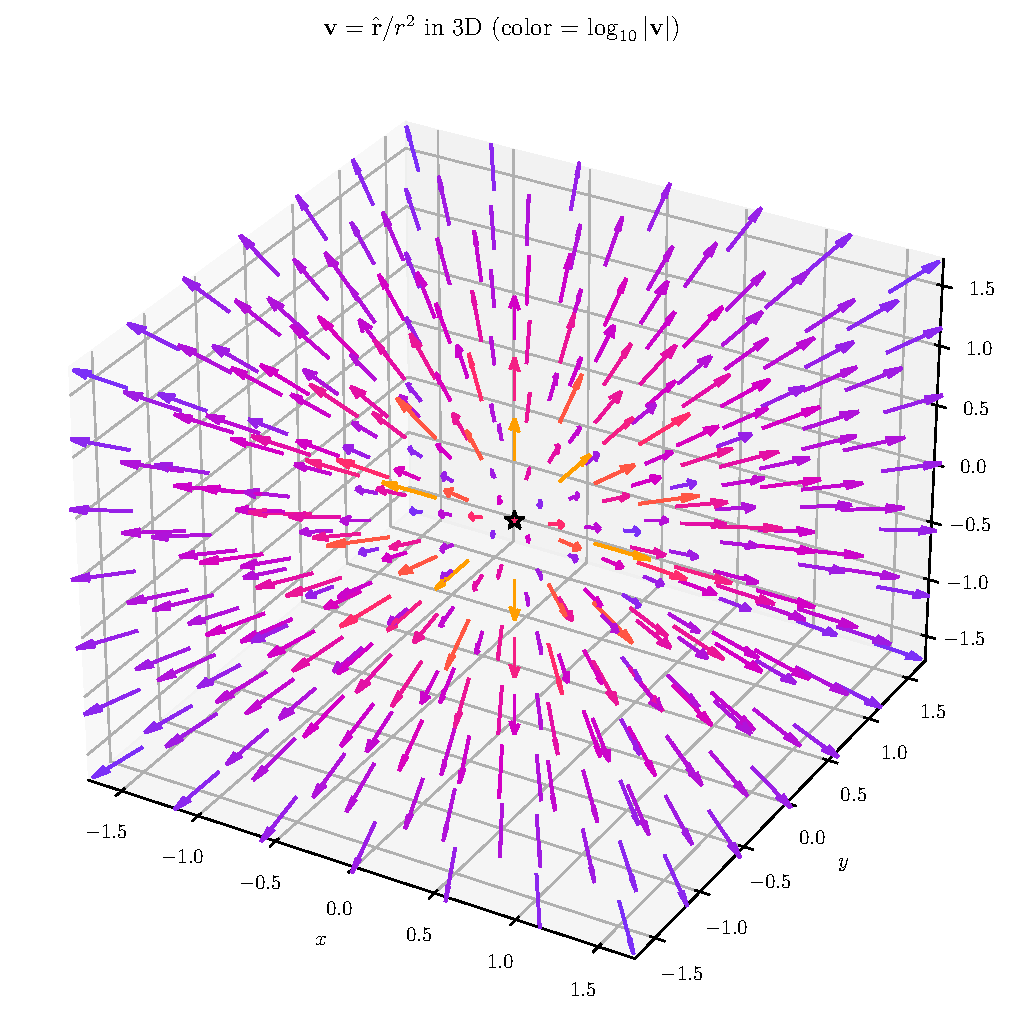
\includegraphics[width=1.0\textwidth]{../chap1/sec1.2/ex1.16.pdf}
\end{center}
Let 
\[
	r = \sqrt{x^{2} + y^{2} + z^{2}}, \quad \pmb{\hat{r}} = \frac{x \pmb{\hat{x}} + y \pmb{\hat{y}} + z \pmb{\hat{z}}}{\sqrt{x^{2} + y^{2} + z^{2}}}
\]
Then
\[
	\pmb{v} = \frac{\pmb{\hat{r}}}{r^{2}} = \frac{x \pmb{\hat{x}} + y \pmb{\hat{y}} + z \pmb{\hat{z}}}{\!\left( x^{2} + y^{2} + z^{2} \right)^{3/2}} 
\]
The divergence is computed as 
\begin{align*}
	\nabla \cdot \pmb{v} & = \frac{\partial }{\partial x}\!\left( \frac{x}{\!\left( x^{2} + y^{2} + z^{2} \right)^{3/2}} \right) + \frac{\partial }{\partial y}\!\left( \frac{y}{\!\left( x^{2} + y^{2} + z^{2} \right)^{3/2}} \right) \\
			     & \qquad + \frac{\partial }{\partial z}\!\left( \frac{z}{\!\left( x^{2} + y^{2} + z^{2} \right)^{3/2}} \right) \\
	 & = \frac{\!\left( y^{2} + z^{2} - 2x^{2} \right) + \!\left( x^{2} + z^{2} - 2y^{2} \right) + \!\left( x^{2} + y^{2} - 2z^{2} \right)}{\!\left( x^{2} + y^{2} + z^{2} \right)^{5/2}} \\ 
	 & = 0
\end{align*}
The counterintuitive solution, then, is the radial vector \( \pmb{v} \) \textbf{has vanishing divergence everywhere except the origin}, for this would produce \( 0 / 0 \). The mechanics of the delta function later will enable us to explore this quandary deeper.

\vspace{12pt}

% QUESTION 17
\qs{1.17}{In two dimensions, show that the divergence transforms as a scalar under rotations. [\textit{Hint}: Use Eq. 1.29 to determine \( \overline{v}_{y} \) and \( \overline{v}_{z} \), and the method of Prob. 1.14 to calculate the derivatives. Your aim is to show that \( \partial \overline{v}_{y} / \partial \overline{y} + \partial \overline{v}_{z} / \partial \overline{z} = \partial v_{y} / \partial y + \partial v_{z} / \partial z \).]} 

By our rotation matrix equation, the transformed quantities are
\begin{align*}
	\overline{v}_{y} & = v_{y}\cos\!\left(\phi\right) + v_{z}\sin\!\left(\phi\right) \\
	\overline{v}_{z} & = -v_{y}\sin\!\left(\phi\right) + v_{z}\cos\!\left(\phi\right)
\end{align*}
The inverse rotation takes us back to
\begin{align*}
	v_{y} & = \overline{v}_{y}\cos\!\left(\phi\right) - \overline{v}_{z}\sin\!\left(\phi\right) \\
	v_{z} & = \overline{v}_{y}\sin\!\left(\phi\right) + \overline{v}_{z}\cos\!\left(\phi\right)
\end{align*}
Using the chain rule, the derivation for \( \partial \overline{v}_{y} / \partial \overline{y} \) and \( \partial \overline{v}_{z} / \partial \overline{z} \) is
\begin{align*}
	\frac{\partial \overline{v}_{y}}{\partial \overline{y}} & = \frac{\partial \overline{v}_{y}}{\partial v_{y}}\!\left( \frac{\partial v_{y}}{\partial y}\frac{\partial y}{\partial \overline{y}} + \frac{\partial v_{y}}{\partial z}\frac{\partial z}{\partial \overline{y}} \right) + \frac{\partial \overline{v}_{y}}{\partial v_{z}}\!\left( \frac{\partial v_{z}}{\partial y}\frac{\partial y}{\partial \overline{y}} + \frac{\partial v_{z}}{\partial z}\frac{\partial z}{\partial \overline{y}} \right) \\
	\frac{\partial \overline{v}_{z}}{\partial \overline{z}} & = \frac{\partial \overline{v}_{z}}{\partial v_{y}}\!\left( \frac{\partial v_{y}}{\partial y} \frac{\partial y}{\partial \overline{z}} + \frac{\partial v_{y}}{\partial z}\frac{\partial z}{\partial \overline{z}} \right) + \frac{\partial \overline{v}_{z}}{\partial v_{z}}\!\left( \frac{\partial v_{z}}{\partial y}\frac{\partial y}{\partial \overline{z}} + \frac{\partial v_{z}}{\partial z}\frac{\partial z}{\partial \overline{z}} \right)
\end{align*}
From problem 1.14, we have each of \( \partial y / \partial \overline{y} \), \( \partial y / \partial \overline{z} \), \( \partial z / \partial \overline{y} \), and \( \partial z / \partial \overline{z} \). From the rotation equations above, we also have
\[
	\frac{\partial \overline{v}_{y}}{\partial v_{y}} = \cos\!\left(\phi\right), \quad \frac{\partial \overline{v}_{y}}{\partial v_{z}} = \sin\!\left(\phi\right), \quad \frac{\partial \overline{v}_{z}}{\partial v_{y}} = -\sin\!\left(\phi\right), \quad \frac{\partial \overline{v}_{z}}{\partial v_{z}} = \cos\!\left(\phi\right)
\]
Combining our ingredients and invoking the Pythagorean theorem, conclude
\begin{align*}
	\frac{\partial \overline{v}_{y}}{\partial \overline{y}} & = \frac{\partial v_{y}}{\partial y}\cos^{2}\!\left(\phi\right) + \frac{\partial v_{y}}{\partial z}\sin\!\left(\phi\right)\cos\!\left(\phi\right) \\
								& \qquad + \frac{\partial v_{z}}{\partial y}\sin\!\left(\phi\right)\cos\!\left(\phi\right) + \frac{\partial v_{z}}{\partial z}\sin^{2}\!\left(\phi\right) \\
	\frac{\partial \overline{v}_{z}}{\partial \overline{z}} & = \frac{\partial v_{z}}{\partial z}\cos^{2}\!\left(\phi\right) - \frac{\partial v_{y}}{\partial z}\sin\!\left(\phi\right)\cos\!\left(\phi\right) \\
								& \qquad - \frac{\partial v_{z}}{\partial y}\sin\!\left(\phi\right)\cos\!\left(\phi\right) + \frac{\partial v_{y}}{\partial y}\sin^{2}\!\left(\phi\right) \\
	\implies \frac{\partial \overline{v}_{y}}{\partial \overline{y}} + \frac{\partial \overline{v}_{z}}{\partial \overline{z}} & = \frac{\partial v_{y}}{\partial y} + \frac{\partial v_{z}}{\partial z}
\end{align*}

\subsubsection{\textsf{1.2.5 - The Curl}}
% QUESTION 18
\qs{1.18}{Calculate the curls of the vector functions in Prob. 1.15.}

\begin{enumerate}[label=(\alph*)]
	\item \begin{align*}
		\nabla \times \pmb{v}_{a} & = \begin{vmatrix}
			\pmb{\hat{x}} & \pmb{\hat{y}} & \pmb{\hat{z}} \\
			\partial / \partial x & \partial / \partial y & \partial / \partial z \\
			x^{2} & 3xz^{2} & -2xz
		\end{vmatrix} \\
		& = \!\left[ \frac{\partial }{\partial y}\!\left( -2xz \right) - \frac{\partial }{\partial z}\!\left( 3xz^{2} \right)\right]\pmb{\hat{x}} + \!\left[ \frac{\partial }{\partial z}\!\left( x^{2} \right) - \frac{\partial }{\partial x}\!\left( -2xz \right) \right]\pmb{\hat{y}} \\
		& \qquad + \!\left[ \frac{\partial }{\partial x}\!\left( 3xz^{2} \right) - \frac{\partial }{\partial y}\!\left( x^{2} \right) \right]\pmb{\hat{z}} \\
		& = -6xz \pmb{\hat{x}} + 2z \pmb{\hat{y}} + 3z^{2}\pmb{\hat{z}}
	\end{align*}
	\item \begin{align*}
		\nabla \times \pmb{v}_{b} & = \begin{vmatrix}
			\pmb{\hat{x}} & \pmb{\hat{y}} & \pmb{\hat{z}} \\
			\partial / \partial x & \partial / \partial y & \partial / \partial z \\
			xy & 2yz & 3zx
		\end{vmatrix} \\
					  & = \!\left[ \frac{\partial }{\partial y}\!\left( 3zx \right) - \frac{\partial }{\partial z}\!\left( 2yz \right) \right]\pmb{\hat{x}} + \!\left[ \frac{\partial }{\partial z}\!\left( xy \right) - \frac{\partial }{\partial x}\!\left( 3zx \right) \right]\pmb{\hat{y}} \\
					  & \qquad + \!\left[ \frac{\partial }{\partial x}\!\left( 2yz \right) - \frac{\partial }{\partial y}\!\left( xy \right) \right]\pmb{\hat{z}} \\
					  & = -2y \pmb{\hat{x}} - 3z \pmb{\hat{y}} - x \pmb{\hat{z}}
	\end{align*}
	\item \begin{align*}
		\nabla \times \pmb{v}_{c} & = \begin{vmatrix}
			\pmb{\hat{x}} & \pmb{\hat{y}} & \pmb{\hat{z}} \\
			\partial / \partial x & \partial / \partial y & \partial / \partial z \\
			y^{2} & 2xy + z^{2} & 2yz
		\end{vmatrix} \\
					  & = \!\left[ \frac{\partial }{\partial y}\!\left( 2yz \right) - \frac{\partial }{\partial z}\!\left( 2xy + z^{2} \right) \right]\pmb{\hat{x}} + \!\left[ \frac{\partial }{\partial z}\!\left( y^{2} \right) - \frac{\partial }{\partial x}\!\left( 2yz \right) \right]\pmb{\hat{y}} \\
					  & \qquad + \!\left[ \frac{\partial }{\partial x}\!\left( 2xy + z^{2} \right) - \frac{\partial }{\partial y}\!\left( y^{2} \right) \right] \\
					  & = \pmb{0}
	\end{align*}
\end{enumerate}

% QUESTION 19
\qs{1.19}{Draw a circle in the \( xy \) plane. At a few representative points draw the vector \( \pmb{v} \) tangent to the circle, pointing in the clockwise direction. By comparing adjacent vectors, determine the \textit{sign} of \( \partial v_{x} / \partial y \) and \( \partial v_{y} / \partial x \). According to Eq. 1.41, then, what is the direction of \( \nabla \times \pmb{v} \)? Explain how this example illustrates the geometrical interpretation of the curl.}

We illustrate tangent vectors pointing clockwise on the unit circle:

\begin{center}
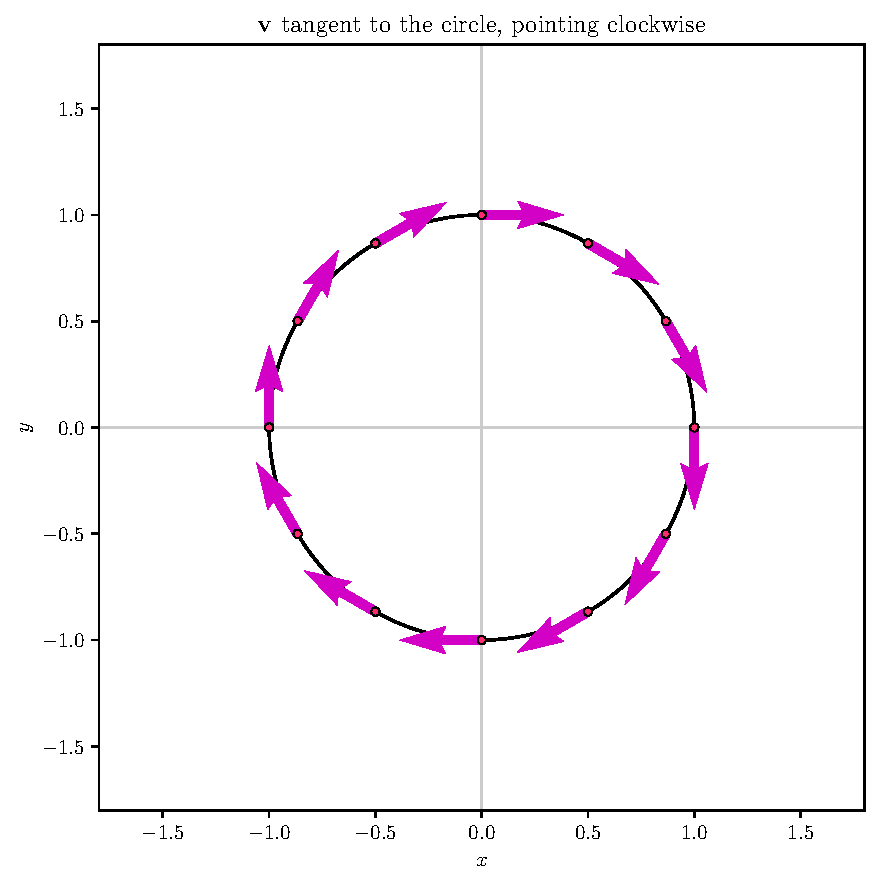
\includegraphics[width=0.5\textwidth]{../chap1/sec1.2/ex1.20.pdf}
\end{center}

Geometrically, observe how as \( x \) increases, the \( v_{y} \) component decreases, and as \( y \) increases, \( v_{x} \) increases. Thus \( \partial v_{x} / \partial y > 0 \) and \( \partial v_{y} / \partial x < 0 \).

Analytically, the vector field describing these tangent clockwise vectors is 
\[
	\pmb{v} = v_{x} \pmb{\hat{x}} + v_{y}\pmb{\hat{y}} = y \pmb{\hat{x}} - x \pmb{\hat{y}} 
\]
Meaning that \( \partial v_{x} / \partial y > 0 \) and \( \partial v_{y} / \partial x < 0 \), and thus \( \partial v_{y} / \partial x -  \partial v_{x} / \partial y < 0 \). This suggests that the curl points in the \textbf{negative} \( z \)-direction.
\[
	\nabla \times \pmb{v} = \!\left( \frac{\partial v_{y}}{\partial x} - \frac{\partial v_{x}}{\partial y} \right)\pmb{\hat{z}} = -2 \pmb{\hat{z}}
\]
By the right-handedness of the coordinate system, this is geometrically intuitive. From our computation of \( \nabla \times \pmb{v} \), we see that the curl is in the negative \( z \)-direction \textit{everywhere}, indicating that if we took any point and applied the right-hand rule, our thumb would point downwards everywhere. 

\vspace{12pt}

% QUESTION 20
\qs{1.20}{Construct a vector function that has zero divergence and zero curl everywhere. (A \textit{constant} will do the job, of course, but make it something a little more interesting than that!)}

Let \( \pmb{v} = v_{x}\pmb{\hat{x}} + v_{y}\pmb{\hat{y}} + v_{z}\pmb{\hat{z}} \). We must find a vector \( \pmb{v} \) whose components satisfy these relations:
\begin{align*}
	\frac{\partial v_{x}}{\partial x} + \frac{\partial v_{y}}{\partial y} + \frac{\partial v_{z}}{\partial z} & = 0 \\
	\frac{\partial v_{z}}{\partial y} - \frac{\partial v_{y}}{\partial z} & = 0 \\ 
	\frac{\partial v_{x}}{\partial z} - \frac{\partial v_{z}}{\partial x} & = 0 \\
	\frac{\partial v_{y}}{\partial x} - \frac{\partial v_{x}}{\partial y} & = 0
\end{align*}

One insight is to realize that if each of the three components are purely in terms of \( x \), \( y \), and \( z \), respectively, then immediately the curl goes to zero. Suppose \( v_{x} = f \!\left( x \right) \), \( v_{y} = g \!\left( y \right) \), and \( v_{z} = h \!\left( z \right) \). Then we need only find functions that satisfy
\[
	\frac{d f}{d x} + \frac{d g}{d y} + \frac{d h}{d z} = 0 
\]
An easy example is: \( f \!\left( x \right) = -x \), \( g \!\left( y \right) = -y \), and \( h \!\left( z \right) = 2z \).

\vspace{12pt}

\subsubsection{\textsf{1.2.6 - Product Rules}}
% QUESTION 21
\qs{1.21}{Prove product rules (i), (iv), and (v).}

(i) \( \nabla \!\left( fg \right) = f \nabla g + g \nabla f \).
\begin{proof}[Proof]
\begin{align*}
	\nabla \!\left( fg \right) & = \frac{\partial }{\partial x}\!\left( fg \right)\pmb{\hat{x}} + \frac{\partial }{\partial y}\!\left( fg \right)\pmb{\hat{y}} + \frac{\partial }{\partial z}\!\left( fg \right)\pmb{\hat{z}} \\
	 & = \!\left( f \frac{\partial g}{\partial x} + g \frac{\partial f}{\partial x} \right)\pmb{\hat{x}} + \!\left( f \frac{\partial g}{\partial y} + g \frac{\partial f}{\partial y} \right)\pmb{\hat{y}} + \!\left( f \frac{\partial g}{\partial z} + g \frac{\partial f}{\partial z} \right)\pmb{\hat{z}} \\
	 & = f \nabla g + g \nabla f
\end{align*}
\end{proof}

(iv) \( \nabla \cdot \!\left( \pmb{A} \times \pmb{B} \right) = \pmb{B} \cdot \!\left( \nabla \times \pmb{A} \right) - \pmb{A} \cdot \!\left( \nabla \times \pmb{B} \right) \).
\begin{proof}[Proof]
First compute \( \pmb{A} \times \pmb{B} \):
\begin{align*}
	\pmb{A} \times \pmb{B} & = \begin{vmatrix}
		\pmb{\hat{x}} & \pmb{\hat{y}} & \pmb{\hat{z}} \\
		A_{x} & A_{y} & A_{z} \\
		B_{x} & B_{y} & B_{z}
	\end{vmatrix} \\
	 & = \!\left( A_{y}B_{z} - A_{z}B_{y} \right)\pmb{\hat{x}} + \!\left( A_{z}B_{x} - A_{x}B_{z} \right)\pmb{\hat{y}} + \!\left( A_{x}B_{y} - A_{y}B_{x} \right)\pmb{\hat{z}}
\end{align*}
Then
\begin{align*}
	\nabla \cdot \!\left( \pmb{A} \times \pmb{B} \right) & = \frac{\partial }{\partial x}\!\left( A_{y}B_{z} - A_{z}B_{y} \right) + \frac{\partial }{\partial y}\!\left( A_{z}B_{x} - A_{x}B_{z} \right) + \frac{\partial }{\partial z}\!\left( A_{x}B_{y} - A_{y}B_{x} \right) \\
	 & = A_{y}\frac{\partial B_{z}}{\partial x} + B_{z}\frac{\partial A_{y}}{\partial x} - A_{z}\frac{\partial B_{y}}{\partial x} - B_{y}\frac{\partial A_{z}}{\partial x} \\ 
	 & \quad + A_{z}\frac{\partial B_{x}}{\partial y} + B_{x}\frac{\partial A_{z}}{\partial y} - A_{x}\frac{\partial B_{z}}{\partial y} - B_{z}\frac{\partial A_{x}}{\partial y} \\
	 & \qquad + A_{x}\frac{\partial B_{y}}{\partial z} + B_{y}\frac{\partial A_{x}}{\partial z} - A_{y}\frac{\partial B_{x}}{\partial z} - B_{x}\frac{\partial A_{y}}{\partial z} \\
	 & = \underbrace{B_{x}\!\left( \frac{\partial A_{z}}{\partial y} - \frac{\partial A_{y}}{\partial z} \right) + B_{y}\!\left( \frac{\partial A_{x}}{\partial z} - \frac{\partial A_{z}}{\partial x} \right) + B_{z}\!\left( \frac{\partial A_{y}}{\partial x} - \frac{\partial A_{x}}{\partial y} \right)}_{\pmb{B} \cdot \!\left( \nabla \times \pmb{A} \right)} \\
	 & + \underbrace{A_{x}\!\left( \frac{\partial B_{z}}{\partial y} - \frac{\partial B_{y}}{\partial z} \right) + A_{y}\!\left( \frac{\partial B_{x}}{\partial z} - \frac{\partial B_{z}}{\partial x} \right) + A_{z}\!\left( \frac{\partial B_{y}}{\partial x} - \frac{\partial B_{x}}{\partial y} \right)}_{\pmb{A} \cdot \!\left( \nabla \times \pmb{B} \right)}
\end{align*}
\end{proof}

(v) \( \nabla \times \!\left( f \pmb{A} \right) = f \!\left( \nabla \times \pmb{A} \right) - \pmb{A} \times \!\left( \nabla f \right) \).

\begin{proof}[Proof]
\begin{align*}
	\nabla \times \!\left( f \pmb{A} \right) & = \begin{vmatrix}
		\pmb{\hat{x}} & \pmb{\hat{y}} & \pmb{\hat{z}} \\
		\frac{\partial }{\partial x} & \frac{\partial }{\partial y} & \frac{\partial }{\partial z} \\
		fA_{x} & fA_{y} & fA_{z}
	\end{vmatrix} \\
						 & = \!\left[ \frac{\partial }{\partial y}\!\left( fA_{z} \right) - \frac{\partial }{\partial z}\!\left( fA_{y} \right) \right]\pmb{\hat{x}} + \!\left[ \frac{\partial }{\partial z}\!\left( fA_{x} \right) - \frac{\partial }{\partial x}\!\left( fA_{z} \right) \right]\pmb{\hat{y}} \\
						 & \quad + \!\left[ \frac{\partial }{\partial x}\!\left( fA_{y} \right) - \frac{\partial }{\partial y}\!\left( fA_{x} \right) \right]\pmb{\hat{z}} \\ 
						 & = \!\left[ f \frac{\partial A_{z}}{\partial y} + A_{z}\frac{\partial f}{\partial y} - f \frac{\partial A_{y}}{\partial z} - A_{y}\frac{\partial f}{\partial z} \right]\pmb{\hat{x}} \\
						 & \quad + \!\left[ f \frac{\partial A_{x}}{\partial z} + A_{x}\frac{\partial f}{\partial z} - f \frac{\partial A_{z}}{\partial x} - A_{z}\frac{\partial f}{\partial x} \right]\pmb{\hat{y}} \\
						 & \qquad + \!\left[ f \frac{\partial A_{y}}{\partial x} + A_{y}\frac{\partial f}{\partial x} - f \frac{\partial A_{x}}{\partial y} - A_{x}\frac{\partial f}{\partial y} \right]\pmb{\hat{z}} \\
						 & = \underbrace{f \!\left[ \!\left( \frac{\partial A_{z}}{\partial y} - \frac{\partial A_{y}}{\partial z} \right)\pmb{\hat{x}} + \!\left( \frac{\partial A_{x}}{\partial z} - \frac{\partial A_{z}}{\partial x} \right)\pmb{\hat{y}} + \!\left( \frac{\partial A_{y}}{\partial x} - \frac{\partial A_{y}}{\partial z} \right)\pmb{\hat{z}} \right]}_{f \!\left( \nabla \times \pmb{A} \right)} \\
						 & \quad - \underbrace{\!\left[  \!\left( A_{y}\frac{\partial f}{\partial z} - A_{z}\frac{\partial f}{\partial y} \right)\pmb{\hat{x}} + \!\left( A_{x}\frac{\partial f}{\partial z} - A_{z}\frac{\partial f}{\partial x} \right)\pmb{\hat{y}} + \!\left( A_{x}\frac{\partial f}{\partial y} - A_{y}\frac{\partial f}{\partial x}\pmb{\hat{z}} \right) \right]}_{\pmb{A} \times \!\left( \nabla f \right)}
\end{align*}
\end{proof}

% QUESTION 22
\qs{1.22}{\begin{enumerate}[label=(\alph*)]
	\item If \( \pmb{A} \) and \( \pmb{B} \) are two vector functions, what does the expression \( \!\left( \pmb{A} \cdot \nabla \right)\pmb{B} \) mean? (That is, what are its \( x \), \( y \), and \( z \) components, in terms of the Cartesian components of \( \pmb{A} \), \( \pmb{B} \), and \( \nabla \)?)
	\item Compute \( \!\left( \pmb{\hat{r}} \cdot \nabla \right)\pmb{\hat{r}} \), where \( \pmb{\hat{r}} \) is the unit vector defined in Eq. 1.21.
	\item For the functions in Prob. 1.15, evaluate \( \!\left( \pmb{v}_{a} \cdot \nabla \right)\pmb{v}_{b} \).
\end{enumerate}}

\begin{enumerate}[label=(\alph*)]
	\item Define \( \pmb{A} = A_{x}\pmb{\hat{x}} + A_{y}\pmb{\hat{y}} + A_{z}\pmb{\hat{z}} \) and \( \pmb{B} = B_{x}\pmb{\hat{x}} + B_{y}\pmb{\hat{y}} + B_{z}\pmb{\hat{z}} \). Then
	\begin{align*}
		\!\left( \pmb{A} \cdot \nabla \right)\pmb{B} & = A_{x}\frac{\partial \pmb{B}}{\partial x} + A_{y}\frac{\partial \pmb{B}}{\partial y} + A_{z}\frac{\partial \pmb{B}}{\partial z} \\
							     & = \sum_{i \in \!\left\{ x,y,z \right\}} \!\left( \sum_{j \in \!\left\{ x,y,z \right\}} A_{j}\frac{\partial B_{i}}{\partial j} \right)\pmb{\hat{i}}
	\end{align*}
	We call this expression the \textbf{directional derivative}.
	\item For \( i,j \in \!\left\{ x,y,z \right\} \), derive
	\[
		\frac{\partial r_{i}}{\partial j} = \begin{cases}
			\displaystyle{\frac{1}{r} - \frac{j^{2}}{r^{3}}} & i = j \\
			\displaystyle{-\frac{ij}{r^{3}}} & i \neq j
		\end{cases}
	\]
	Then we can compute
	\[
		\!\left( \pmb{\hat{r}} \cdot \nabla \right)\pmb{\hat{r}} = \frac{1}{r}\sum_{i \in \!\left\{ x,y,z \right\}}\!\left( \sum_{j \in \!\left\{ x,y,z \right\}} j \frac{\partial r_{i}}{\partial j} \right)\pmb{\hat{i}}
	\]
	Take \( i = x \) to see how this computation works. We have
	\begin{align*}
		\!\left[ \!\left( \pmb{\hat{r}} \cdot \nabla \right)\pmb{\hat{r}} \right]_{x} & = \frac{1}{r}\!\left( x \frac{\partial r_{x}}{\partial x} + y \frac{\partial r_{x}}{\partial y} + z \frac{\partial r_{x}}{\partial z} \right) \\
		& = \frac{1}{r}\!\left[ x\!\left( \frac{1}{r} - \frac{x^{2}}{r^{3}} \right) - \frac{xy^{2}}{r^{3}} - \frac{xz^{2}}{r^{3}} \right] \\ 
		& = \frac{1}{r}\!\left[ x \!\left( \frac{1}{r} - \!\left( \frac{x^{2} + y^{2} + z^{2}}{r^{3}} \right) \right) \right] \\
		& = \frac{1}{r}\!\left[ x \!\left( \frac{1}{r} - \frac{1}{r} \right) \right] \\
		& = 0 
	\end{align*}
	An extraordinary reduction. By symmetry, it follows that the components for \( y \) and \( z \) follow analogously. Then we can conclude
	\[
		\!\left( \pmb{\hat{r}} \cdot \nabla \right)\pmb{\hat{r}} = \pmb{0} 
	\]
	\item \begin{align*}
		\!\left( \pmb{v}_{a} \cdot \nabla \right)\pmb{v}_{b} & = \sum_{i \in \!\left\{ x,y,z \right\}} \!\left( \sum_{j \in \!\left\{ x,y,z \right\}} v_{a,j}\frac{\partial v_{b,i}}{\partial j} \right)\pmb{\hat{i}} \\
		 & = \!\left( x^{2}y + 3x^{2}z^{2} \right)\pmb{\hat{x}} + \!\left( 6xz^{3} - 4xyz \right)\pmb{\hat{y}} - 3x^{2}z \pmb{\hat{z}}
	\end{align*}
\end{enumerate}

% QUESTION 23
\qs{1.23}{(For masochists only.) Prove product rules (ii) and (vi). Refer to Prob. 1.22 for the definition of \( \!\left( \pmb{A} \cdot \nabla \right)\pmb{B} \).}

(ii) \( \nabla \!\left( \pmb{A} \cdot \pmb{B} \right) = \pmb{A} \times \!\left( \nabla \times \pmb{B} \right) + \pmb{B} \times \!\left( \nabla \times \pmb{A} \right) + \!\left( \pmb{A} \cdot \nabla \right)\pmb{B} + \!\left( \pmb{B} \cdot \nabla \right)\pmb{A} \).

\begin{proof}[Proof]
\begin{align*}
	\nabla \!\left( \pmb{A} \cdot \pmb{B} \right) & = \nabla \!\left( A_{x}B_{x} + A_{y}B_{y} + A_{z}B_{z} \right) \\
	 & = \sum_{i \in \!\left\{ x,y,z \right\}} \!\left( \sum_{j \in \!\left\{ x,y,z \right\}} A_{j}\frac{\partial B_{j}}{\partial i} + B_{j}\frac{\partial A_{j}}{\partial i} \right)\pmb{\hat{i}} \\
	\pmb{A} \times \!\left( \nabla \times \pmb{B} \right) & = \begin{vmatrix}
		\pmb{\hat{x}} & \pmb{\hat{y}} & \pmb{\hat{z}} \\
		A_{x} & A_{y} & A_{z} \\
		\frac{\partial B_{z}}{\partial y} - \frac{\partial B_{y}}{\partial z} & \frac{\partial B_{x}}{\partial z} - \frac{\partial B_{z}}{\partial x} & \frac{\partial B_{y}}{\partial x} - \frac{\partial B_{x}}{\partial y}
	\end{vmatrix} \\
							      & = \!\left[ A_{y}\!\left( \textcolor{red}{\frac{\partial B_{y}}{\partial x}} \textcolor{blue}{- \frac{\partial B_{x}}{\partial y}} \right) - A_{z}\!\left( \textcolor{blue}{\frac{\partial B_{x}}{\partial z}} \textcolor{red}{- \frac{\partial B_{z}}{\partial x}} \right) \right]\pmb{\hat{x}} \\
							      & \quad + \!\left[ A_{z}\!\left( \textcolor{red}{\frac{\partial B_{z}}{\partial y}} \textcolor{blue}{- \frac{\partial B_{y}}{\partial z}} \right) - A_{x}\!\left( \textcolor{blue}{\frac{\partial B_{y}}{\partial x}} \textcolor{red}{- \frac{\partial B_{x}}{\partial y}} \right) \right]\pmb{\hat{y}} \\
							      & \qquad + \!\left[ A_{x}\!\left( \textcolor{red}{\frac{\partial B_{x}}{\partial z}} \textcolor{blue}{- \frac{\partial B_{z}}{\partial x}} \right) - A_{y}\!\left( \textcolor{blue}{\frac{\partial B_{z}}{\partial y}} \textcolor{red}{- \frac{\partial B_{y}}{\partial z}} \right) \right]\pmb{\hat{z}} \\
	\pmb{B} \times \!\left( \nabla \times \pmb{A} \right) & = \begin{vmatrix}
		\pmb{\hat{x}} & \pmb{\hat{y}} & \pmb{\hat{z}} \\
		B_{x} & B_{y} & B_{z} \\
		\frac{\partial A_{z}}{\partial y} - \frac{\partial A_{y}}{\partial z} & \frac{\partial A_{x}}{\partial z} - \frac{\partial A_{z}}{\partial x} & \frac{\partial A_{y}}{\partial x} - \frac{\partial A_{x}}{\partial y}
	\end{vmatrix} \\
							      & = \!\left[ B_{y}\!\left( \textcolor{red}{\frac{\partial A_{y}}{\partial x}} \textcolor{blue}{- \frac{\partial A_{x}}{\partial y}} \right) - B_{z}\!\left( \textcolor{blue}{\frac{\partial A_{x}}{\partial z}} \textcolor{red}{- \frac{\partial A_{z}}{\partial x}} \right) \right]\pmb{\hat{x}} \\
							      & \quad + \!\left[ B_{z}\!\left( \textcolor{red}{\frac{\partial A_{z}}{\partial y}} \textcolor{blue}{- \frac{\partial A_{y}}{\partial z}} \right) - B_{x}\!\left( \textcolor{blue}{\frac{\partial A_{y}}{\partial x}} \textcolor{red}{- \frac{\partial A_{x}}{\partial y}} \right) \right]\pmb{\hat{y}} \\
							      & \qquad + \!\left[ B_{x}\!\left( \textcolor{red}{\frac{\partial A_{x}}{\partial z}} \textcolor{blue}{- \frac{\partial A_{z}}{\partial x}} \right) - B_{y}\!\left( \textcolor{blue}{\frac{\partial A_{z}}{\partial y}} \textcolor{red}{- \frac{\partial A_{y}}{\partial z}} \right) \right]\pmb{\hat{z}} \\
	\!\left( \pmb{A} \cdot \nabla \right)\pmb{B} & = \sum_{i \in \!\left\{ x,y,z \right\}} \!\left( \sum_{j \in \!\left\{ x,y,z \right\}} A_{j}\frac{\partial B_{i}}{\partial j} \right)\pmb{\hat{i}} \\
	\!\left( \pmb{B} \cdot \nabla \right)\pmb{A} & = \sum_{i \in \!\left\{ x,y,z \right\}} \!\left( \sum_{j \in \!\left\{ x,y,z \right\}} B_{j}\frac{\partial A_{i}}{\partial j} \right)\pmb{\hat{i}}
\end{align*}

Adding \( \pmb{A} \times \!\left( \nabla \times \pmb{B} \right) \) and \( \pmb{B} \times \!\left( \nabla \times \pmb{A} \right) \), derive
\begin{align*}
	\textcolor{red}{\sum_{i \in \!\left\{ x,y,z \right\}}} & \textcolor{red}{\!\left( \sum_{j \in \!\left\{ x,y,z \right\}} \!\left( 1 - \delta_{ij} \right)\!\left( A_{j}\frac{\partial B_{j}}{\partial i} + B_{j}\frac{\partial A_{j}}{\partial i} \right) \right)\pmb{\hat{i}}} \\
							       & \textcolor{blue}{-\sum_{i \in \!\left\{ x,y,z \right\}} \!\left( \sum_{j \in \!\left\{ x,y,z \right\}} \!\left( 1 - \delta_{ij} \right)\!\left( A_{j}\frac{\partial B_{i}}{\partial j} + B_{j}\frac{\partial A_{i}}{\partial j} \right) \right) \pmb{\hat{i}}}
\end{align*}

Now, looking at the directional derivatives, we may write their sum \( \!\left( \pmb{A} \cdot \nabla \right)\pmb{B} + \!\left( \pmb{B} \cdot \nabla \right)\pmb{A} \) as 
\[
	\textcolor{red}{\sum_{i \in \!\left\{ x,y,z \right\}} \!\left( A_{i}\frac{\partial B_{i}}{\partial i} + B_{i}\frac{\partial A_{i}}{\partial i} \right)\pmb{\hat{i}}} \textcolor{blue}{+ \sum_{i \in \!\left\{ x,y,z \right\}} \!\left( \sum_{j \in \!\left\{ x,y,z \right\}} \!\left( 1 - \delta_{ij} \right)\!\left( A_{j}\frac{\partial B_{i}}{\partial j} + B_{j}\frac{\partial A_{i}}{\partial j} \right) \right) \pmb{\hat{i}}}
\]
The blue summations cancel each other out, while the red terms sum to the desired result. Observe that the heart of the proof arose in decomposing the derivative structures: the first corresponds to the gradient and the second to the directional derivative.
\[
	A_{\textcolor{red}{j}}\frac{\partial B_{\textcolor{red}{j}}}{\partial i} \text{ (gradient)} \qquad A_{\textcolor{red}{j}}\frac{\partial B_{i}}{\partial \textcolor{red}{j}} \text{ (directional derivative)}
\]
\end{proof}

(vi) \( \nabla \times \!\left( \pmb{A} \times \pmb{B} \right) = \!\left( \pmb{B} \cdot \nabla \right)\pmb{A} - \!\left( \pmb{A} \cdot \nabla \right)\pmb{B} + \pmb{A}\!\left( \nabla \cdot \pmb{B} \right) - \pmb{B}\!\left( \nabla \cdot \pmb{A} \right) \).

\begin{proof}[Proof]
\begin{align*}
	\nabla \times \!\left( \pmb{A} \times \pmb{B} \right) & = \begin{vmatrix}
		\pmb{\hat{x}} & \pmb{\hat{y}} & \pmb{\hat{z}} \\[3pt]
		\frac{\partial }{\partial x} & \frac{\partial }{\partial y} & \frac{\partial }{\partial z} \\[6pt]
		A_{y}B_{z} - A_{z}B_{y} & A_{z}B_{x} - A_{x}B_{z} & A_{x}B_{y} - A_{y}B_{x}
	\end{vmatrix} \\
							      & = \sum_{i \in \!\left\{ x,y,z \right\}}\!\left\{ \sum_{j \in \!\left\{ x,y,z \right\}} \!\left[ \!\left( \textcolor{red}{A_{i}\frac{\partial B_{j}}{\partial j}} + \textcolor{blue}{B_{j}\frac{\partial A_{i}}{\partial j}} \right) - \!\left( \textcolor{blue}{A_{j}\frac{\partial B_{i}}{\partial j}} + \textcolor{red}{B_{i}\frac{\partial A_{j}}{\partial j}} \right) \right]\right\}\pmb{\hat{i}} \\
		\!\left( \pmb{B} \cdot \nabla \right)\pmb{A} & = \sum_{i \in \!\left\{ x,y,z \right\}} \!\left( \sum_{j \in \!\left\{ x,y,z \right\}} \textcolor{blue}{B_{j}\frac{\partial A_{i}}{\partial j}} \right)\pmb{\hat{i}} \\
		\!\left( \pmb{A} \cdot \nabla \right)\pmb{B} & = \sum_{i \in \!\left\{ x,y,z \right\}} \!\left( \sum_{j \in \!\left\{ x,y,z \right\}} \textcolor{blue}{A_{j}\frac{\partial B_{i}}{\partial j}} \right)\pmb{\hat{i}} \\
		\pmb{A}\!\left( \nabla \cdot \pmb{B} \right) & = \sum_{i \in \!\left\{ x,y,z \right\}} \!\left( \sum_{j \in \!\left\{ x,y,z \right\}} \textcolor{red}{A_{i}\frac{\partial B_{j}}{\partial j}} \right)\pmb{\hat{i}} \\
		\pmb{B}\!\left( \nabla \cdot \pmb{A} \right) & = \sum_{i \in \!\left\{ x,y,z \right\}} \!\left( \sum_{j \in \!\left\{ x,y,z \right\}} \textcolor{red}{B_{i}\frac{\partial A_{j}}{\partial j}} \right)\pmb{\hat{i}}
\end{align*}
Where once again, we combine \textcolor{red}{divergence} and \textcolor{blue}{directional derivative} components to produce the desired result.
\end{proof}

% QUESTION 24
\qs{1.24}{Derive the three quotient rules.}

Switch either \( g \rightarrow g^{-1} \) or \( f \rightarrow f^{-1} \) to find

\begin{align*}
	\nabla \!\left( \frac{f}{g} \right) & = \nabla \!\left( fg^{-1} \right) \\
					    & = f \nabla g^{-1} + g^{-1}\nabla f \\
					    & = \frac{g \nabla f - f \nabla g}{g^{2}} \\
	\nabla \cdot \!\left( \frac{1}{f} \pmb{A} \right) & = \nabla \cdot \!\left( f^{-1}\pmb{A} \right) \\
							  & = f^{-1}\!\left( \nabla \cdot \pmb{A} \right) + \pmb{A} \cdot \!\left( \nabla f^{-1} \right) \\
							  & = \frac{f \!\left( \nabla \cdot \pmb{A} \right) - \pmb{A} \cdot \nabla f}{f^{2}} \\
	\nabla \times \!\left( \frac{1}{f}\pmb{A} \right) & = \nabla \times \!\left( f^{-1}\pmb{A} \right) \\
							  & = f^{-1}\!\left( \nabla \times \pmb{A} \right) - \pmb{A} \times \!\left( \nabla f^{-1} \right) \\
							  & = \frac{f \!\left( \nabla \times \pmb{A} \right) + \pmb{A} \times \nabla f}{f^{2}}
\end{align*}

% QUESTION 25
\qs{1.25}{\begin{enumerate}[label=(\alph*)]
	\item Check product rule (iv) (by calculating each term separately) for the functions
	\[
		\pmb{A} = x \pmb{\hat{x}} + 2y \pmb{\hat{y}} + 3z \pmb{\hat{z}} \qquad \pmb{B}= 3y \pmb{\hat{x}} - 2x \pmb{\hat{y}} 
	\]
	\item Do the same for product rule (ii).
	\item Do the asme for rule (vi).
\end{enumerate}}

Use the fact that \( \nabla \times A = \pmb{0} \) from our insight in problem 1.20 that a zero curl arises when each component function is strictly in the variable of its corresponding basis coordinate.

\begin{enumerate}[label=(\alph*)]
	\item \begin{align*}
		\pmb{A} \times \pmb{B} & = \begin{vmatrix}
			\pmb{\hat{x}} & \pmb{\hat{y}} & \pmb{\hat{z}} \\
			x & 2y & 3z \\
			3y & -2x & 0
		\end{vmatrix} \\
				       & = 6xz \pmb{\hat{x}} + 9yz \pmb{\hat{y}} - \!\left(2x^{2} + 6y^{2} \right)\pmb{\hat{z}} \\
	\boxed{\nabla \cdot \!\left( \pmb{A} \times \pmb{B} \right)} & = \frac{\partial }{\partial x}\!\left( 6xz \right) + \frac{\partial }{\partial y}\!\left( 9yz \right) - \frac{\partial }{\partial z}\!\left( 2x^{2} + 6y^{2} \right) \\
								     & = \boxed{15z} \\
	\boxed{\pmb{B} \cdot \!\left( \nabla \times \pmb{A} \right)} & = \boxed{0} \\
					       \nabla \times \pmb{B} & = \begin{vmatrix}
					       	\pmb{\hat{x}} & \pmb{\hat{y}} & \pmb{\hat{z}} \\
					       	\frac{\partial }{\partial x} & \frac{\partial }{\partial y} & \frac{\partial }{\partial z} \\
					       	3y & -2x & 0
					       \end{vmatrix} \\
								     & = -5 \pmb{\hat{z}} \\
			\boxed{\pmb{A} \cdot \!\left( \nabla \times \pmb{B} \right)} & = \boxed{-15z} \\
			\boxed{\pmb{B} \cdot \!\left( \nabla \times \pmb{A} \right) - \pmb{A} \cdot \!\left( \nabla \times \pmb{B} \right)} & = \boxed{15z}
	\end{align*}
	\item \begin{align*}
			\boxed{\nabla \!\left( \pmb{A} \cdot \pmb{B} \right)} & = \frac{\partial }{\partial x}\!\left( -xy \right)\pmb{\hat{x}} + \frac{\partial }{\partial y}\!\left( -xy \right)\pmb{\hat{y}} \\
									      & = \boxed{-y \pmb{\hat{x}} - x \pmb{\hat{y}}} \\
							\nabla \times \pmb{B} & = -5 \pmb{\hat{z}} \\
							\boxed{\pmb{A} \times \!\left( \nabla \times \pmb{B} \right)} & = \begin{vmatrix}
								\pmb{\hat{x}} & \pmb{\hat{y}} & \pmb{\hat{z}} \\
								x & 2y & 3z \\
								0 & 0 & -5
							\end{vmatrix} \\
														      & = \boxed{-10y \pmb{\hat{x}} + 5x \pmb{\hat{y}}} \\
								\boxed{\pmb{B} \times \!\left( \nabla \times \pmb{A} \right)} & = \boxed{\pmb{0}} \\
								\boxed{\!\left( \pmb{A} \cdot \nabla \right)\pmb{B}} & = x \frac{\partial \pmb{B}}{\partial x} + 2y \frac{\partial \pmb{B}}{\partial y} \\
														     & = \boxed{6y \pmb{\hat{x}} - 2x \pmb{\hat{y}}} \\
								\boxed{\!\left( \pmb{B} \cdot \nabla \right)\pmb{A}} & = 3y \frac{\partial \pmb{A}}{\partial x} - 2x \frac{\partial \pmb{A}}{\partial y} \\
														     & = \boxed{3y \pmb{\hat{x}} - 4x \pmb{\hat{y}}}
\end{align*}
Summing our terms together, derive
\[
	\pmb{A} \times \!\left( \nabla \times \pmb{B} \right) + \pmb{B} \times \!\left( \nabla \times \pmb{A} \right) + \!\left( \pmb{A} \cdot \nabla \right)\pmb{B} + \!\left( \pmb{B} \cdot \nabla \right)\pmb{A} = \boxed{-y \pmb{\hat{x}} - x \pmb{\hat{y}}}
\]
	\item \begin{align*}
		\boxed{\nabla \times \!\left( \pmb{A} \times \pmb{B} \right)} & = \begin{vmatrix}
			\pmb{\hat{x}} & \pmb{\hat{y}} & \pmb{\hat{z}} \\
			\frac{\partial }{\partial x} & \frac{\partial }{\partial y} & \frac{\partial }{\partial z} \\
			6xz & 9yz & -\!\left( 2x^{2} + 6y^{2} \right)
		\end{vmatrix} \\
									      & = \!\left[ \frac{\partial }{\partial y}\!\left[ -\!\left( 2x^{2} + 6y^{2} \right)\right] - \frac{\partial }{\partial z}\!\left( 9yz \right) \right]\pmb{\hat{x}} \\
									      & \quad + \!\left[ \frac{\partial }{\partial z}\!\left( 6xz \right) + \frac{\partial }{\partial x}\!\left( 2x^{2} + 6y^{2} \right) \right]\pmb{\hat{y}} \\ 
									      & \qquad + \!\left[ \frac{\partial }{\partial x}\!\left( 9yz \right) - \frac{\partial }{\partial y}\!\left( 6xz \right) \right]\pmb{\hat{z}} \\
									      & = \boxed{-21y \pmb{\hat{x}} + 10x \pmb{\hat{y}}} \\ 
			\boxed{\!\left( \pmb{B} \cdot \nabla \right)\pmb{A}} & = \boxed{3y \pmb{\hat{x}} - 4x \pmb{\hat{y}}} \\
			\boxed{\!\left( \pmb{A} \cdot \nabla \right)\pmb{B}} & = \boxed{6y \pmb{\hat{x}} - 2x \pmb{\hat{y}}} \\
			\boxed{\pmb{A}\!\left( \nabla \cdot \pmb{B} \right)} & = \boxed{\pmb{0}} \\
			\boxed{\pmb{B}\!\left( \nabla \cdot \pmb{A} \right)} & = 6 \pmb{B} \\
									     & = \boxed{18y \pmb{\hat{x}} - 12x \pmb{\hat{y}}}
	\end{align*}
	Combining the last four terms as rule (vi) stipulates, we have
	\[
		\!\left( \pmb{B} \cdot \nabla \right)\pmb{A} - \!\left( \pmb{A} \cdot \nabla \right)\pmb{B} + \pmb{A}\!\left( \nabla \cdot \pmb{B} \right) - \pmb{B}\!\left( \nabla \cdot \pmb{A} \right) = -21y \pmb{\hat{x}} + 10x \pmb{\hat{y}} 
	\]
\end{enumerate}

\subsubsection{\textsf{1.2.7 - Second Derivatives}}
% QUESTION 26
\qs{1.26}{Calculate the Laplacian of the following functions:
\begin{enumerate}[label=(\alph*)]
	\item \( T_{a} = x^{2} + 2xy + 3z + 4 \)
	\item \( T_{b} = \sin\!\left(x\right)\sin\!\left(y\right)\sin\!\left(z\right) \)
	\item \( T_{c} = e^{-5x}\sin\!\left(4y\right)\cos\!\left(3z\right) \)
	\item \( \pmb{v} = x^{2}\pmb{\hat{x}} + 3xz^{2}\pmb{\hat{y}} - 2xz \pmb{\hat{z}} \)
\end{enumerate}}

\begin{enumerate}[label=(\alph*)]
	\item \[
		\nabla^{2}T_{a} = \frac{\partial^2 T_{a}}{\partial x^2} + \frac{\partial^2 T_{a}}{\partial y^2} + \frac{\partial^2 T_{a}}{\partial z^2} = 2
	\]
	\item \[
		\nabla^{2}T_{b} = \frac{\partial^2 T_{b}}{\partial x^2} + \frac{\partial^2 T_{b}}{\partial y^2} + \frac{\partial^2 T_{b}}{\partial z^2} = -3 \sin\!\left(x\right)\sin\!\left(y\right)\sin\!\left(z\right)
	\]
	\item \[
		\nabla^{2}T_{c} = \frac{\partial^2 T_{c}}{\partial x^2} + \frac{\partial^2 T_{c}}{\partial y^2} + \frac{\partial^2 T_{c}}{\partial z^2} = \!\left( 25 - 16 - 3 \right)e^{-5x}\sin\!\left(4y\right)\cos\!\left(3z\right) = 0 
	\]
	\item \[
		\nabla^{2}\pmb{v} = \nabla^{2}\!\left( x^{2} \right)\pmb{\hat{x}} + \nabla^{2}\!\left( 3xz^{2} \right)\pmb{\hat{y}} + \nabla^{2}\!\left( -2xz \right)\pmb{\hat{z}} = 2 \pmb{\hat{x}} + 6x \pmb{\hat{y}}
	\]
\end{enumerate}

% QUESTION 27
\qs{1.27}{Prove that the divergence of a curl is always zero. \textit{Check} it for function \( \pmb{v}_{a} \) in Prob. 1.15.}

\( \nabla \cdot \!\left( \nabla \times \pmb{v} \right) = 0 \).

\begin{proof}[Proof]
\begin{align*}
	\nabla \times \pmb{v} & = \begin{vmatrix}
		\pmb{\hat{x}} & \pmb{\hat{y}} & \pmb{\hat{z}} \\
		\frac{\partial }{\partial x} & \frac{\partial }{\partial y} & \frac{\partial }{\partial z} \\
		v_{x} & v_{y} & v_{z}
	\end{vmatrix} \\
	 & = \!\left( \frac{\partial v_{z}}{\partial y} - \frac{\partial v_{y}}{\partial z} \right)\pmb{\hat{x}} + \!\left( \frac{\partial v_{x}}{\partial z} - \frac{\partial v_{z}}{\partial x} \right)\pmb{\hat{y}} + \!\left( \frac{\partial v_{y}}{\partial x} - \frac{\partial v_{x}}{\partial y} \right)\pmb{\hat{z}} \\ 
		\nabla \cdot \!\left( \nabla \times \pmb{v} \right) & = \frac{\partial }{\partial x}\!\left( \textcolor{red}{\frac{\partial v_{z}}{\partial y}} - \textcolor{blue}{\frac{\partial v_{y}}{\partial z}} \right) + \frac{\partial }{\partial y}\!\left( \textcolor{green}{\frac{\partial v_{x}}{\partial z}} - \textcolor{red}{\frac{\partial v_{z}}{\partial x}} \right) + \frac{\partial }{\partial z}\!\left( \textcolor{blue}{\frac{\partial v_{y}}{\partial x}} - \textcolor{green}{\frac{\partial v_{x}}{\partial y}} \right)
\end{align*}
By Clairaut's theorem, assuming continuity of the mixed second partial derivatives, the differentiation is agnostic of order:
\[
	\frac{\partial^{2} v_{i}}{\partial j \partial k} = \frac{\partial^{2} v_{i}}{\partial k \partial j} 
\]
where the three colored pairs (after distribution) cancel pursuant to Clairaut's theorem. 
\end{proof}
Using \( \pmb{v} = \pmb{v}_{a} \), we have
\begin{align*}
	\nabla \times \pmb{v}_{a} & = \begin{vmatrix}
		\pmb{\hat{x}} & \pmb{\hat{y}} & \pmb{\hat{z}} \\
		\frac{\partial }{\partial x} & \frac{\partial }{\partial y} & \frac{\partial }{\partial z} \\
		x^{2} & 3xz^{2} & -2xz
	\end{vmatrix} \\
	 & = -6xz \pmb{\hat{x}} + 2z \pmb{\hat{y}} + 3z^{2}\pmb{\hat{z}} \\ 
		\nabla \cdot \!\left( \nabla \times \pmb{v}_{a} \right) & = \frac{\partial }{\partial x}\!\left( -6xz \right) + \frac{\partial }{\partial y}\!\left( 2z \right) + \frac{\partial }{\partial z}\!\left( 3z^{2} \right) \\
									& = 0
\end{align*}

% QUESTION 28
\qs{1.28}{Prove that the curl of a gradient is always zero. \textit{Check} it for function (b) in Prob. 1.11.}

\( \nabla \times \!\left( \nabla T \right) = \pmb{0} \).
\begin{proof}[Proof]
\begin{align*}
	\nabla \times \!\left( \nabla T \right) & = \begin{vmatrix}
		\pmb{\hat{x}} & \pmb{\hat{y}} & \pmb{\hat{z}} \\[3pt]
		\frac{\partial }{\partial x} & \frac{\partial }{\partial y} & \frac{\partial }{\partial z} \\[6pt]
		\frac{\partial T}{\partial x} & \frac{\partial T}{\partial y} & \frac{\partial T}{\partial z}
	\end{vmatrix} \\
	 & = \!\left( \frac{\partial^{2}T}{\partial y \partial z} - \frac{\partial^{2}T}{\partial z \partial y} \right)\pmb{\hat{x}} + \!\left( \frac{\partial^{2}T}{\partial z \partial x} - \frac{\partial^{2}T}{\partial x \partial z} \right)\pmb{\hat{y}} + \!\left( \frac{\partial^{2}T}{\partial x \partial y} - \frac{\partial^{2}T}{\partial y \partial x} \right)\pmb{\hat{z}} \\
	 & = \pmb{0}
\end{align*}
where the last equality follows from Clairaut's theorem.
\end{proof}
Using \( f \!\left( x,y,z \right) = x^{2}y^{3}z^{4} \), calculate
\begin{align*}
	\nabla f & = 2xy^{3}z^{4}\pmb{\hat{x}} + 3x^{2}y^{2}z^{4}\pmb{\hat{y}} + 4x^{2}y^{3}z^{3}\pmb{\hat{z}} \\
	\nabla \times \!\left( \nabla f \right) & = \begin{vmatrix}
		\pmb{\hat{x}} & \pmb{\hat{y}} & \pmb{\hat{z}} \\[3pt]
		\frac{\partial }{\partial x} & \frac{\partial }{\partial y} & \frac{\partial }{\partial z} \\[6pt]
		2xy^{3}z^{4} & 3x^{2}y^{2}z^{4} & 4x^{2}y^{3}z^{3} \\
	\end{vmatrix} \\
						& = \!\left[ \frac{\partial }{\partial y}\!\left( 4x^{2}y^{3}z^{3} \right) - \frac{\partial }{\partial z}\!\left( 3x^{2}y^{2}z^{4} \right) \right]\pmb{\hat{x}} \\
						& + \quad \!\left[ \frac{\partial }{\partial z}\!\left( 2xy^{3}z^{4} \right) - \frac{\partial }{\partial x}\!\left( 4x^{2}y^{3}z^{3} \right) \right]\pmb{\hat{y}} \\
						& \qquad + \!\left[ \frac{\partial }{\partial x}\!\left( 3x^{2}y^{2}z^{4} \right) - \frac{\partial }{\partial y}\!\left( 2xy^{3}z^{4} \right) \right]\pmb{\hat{z}} \\
						& = \pmb{0}
\end{align*}

\newpage

\subsection{\textsf{1.3 - Integral Calculus}}
\subsubsection{\textsf{1.3.1 - Line, Surface, and Volume Integrals}}
% QUESTION 29
\qs{1.29}{Calculate the line integral of the function \( \pmb{v} = x^{2}\pmb{\hat{x}} + 2yz \pmb{\hat{y}} + y^{2}\pmb{\hat{z}} \) from the origin to the point \( \!\left( 1,1,1 \right) \) by three different routes:
\begin{enumerate}[label=(\alph*)]
	\item \( \!\left( 0,0,0 \right) \rightarrow \!\left( 1,0,0 \right) \rightarrow \!\left( 1,1,0 \right) \rightarrow \!\left( 1,1,1 \right) \).
	\item \( \!\left( 0,0,0 \right) \rightarrow \!\left( 0,0,1 \right) \rightarrow \!\left( 0,1,1 \right) \rightarrow \!\left( 1,1,1 \right) \).
	\item The direct straight line.
	\item What is the line integral around the closed loop that goes \textit{out} along path (a) and \textit{back} along path (b)?
\end{enumerate}}

\begin{figure}[h]
\centering
% ---- Path (a): (0,0,0)->(1,0,0)->(1,1,0)->(1,1,1) ----
\begin{tikzpicture}[scale=1.6,
    axisstyle/.style={->, gray, thin},
    pathstyle/.style={->, thick, blue},
    vertex/.style={circle, fill=black, inner sep=1pt}]
  % axes (x to the right-front, y to the right-back, z up)
  \coordinate (O) at (0,0,0);
  \draw[axisstyle] (O) -- (1.5,0,0) node[right] {\footnotesize $x$};
  \draw[axisstyle] (O) -- (0,1.5,0) node[above] {\footnotesize $z$};
  \draw[axisstyle] (O) -- (0,0,1.5) node[below left] {\footnotesize $y$};
  % path vertices
  \coordinate (P0) at (0,0,0);
  \coordinate (P1) at (1,0,0);
  \coordinate (P2) at (1,0,1);
  \coordinate (P3) at (1,1,1);
  % path
  \draw[pathstyle] (P0) -- (P1) -- (P2) -- (P3);
  % dots + labels
  \node[vertex] at (P0) {}; \node[below left]  at (P0) {\scriptsize $(0,0,0)$};
  \node[vertex] at (P1) {}; \node[below right] at (P1) {\scriptsize $(1,0,0)$};
  \node[vertex] at (P2) {}; \node[right]       at (P2) {\scriptsize $(1,1,0)$};
  \node[vertex] at (P3) {}; \node[above right] at (P3) {\scriptsize $(1,1,1)$};
  \node at (0.75,-0.55,0) {\small (a)};
\end{tikzpicture}
\hfill
% ---- Path (b): (0,0,0)->(0,0,1)->(0,1,1)->(1,1,1) ----
\begin{tikzpicture}[scale=1.6,
    axisstyle/.style={->, gray, thin},
    pathstyle/.style={->, thick, red},
    vertex/.style={circle, fill=black, inner sep=1pt}]
  \coordinate (O) at (0,0,0);
  \draw[axisstyle] (O) -- (1.5,0,0) node[right] {\footnotesize $x$};
  \draw[axisstyle] (O) -- (0,1.5,0) node[above] {\footnotesize $z$};
  \draw[axisstyle] (O) -- (0,0,1.5) node[below left] {\footnotesize $y$};
  \coordinate (P0) at (0,0,0);
  \coordinate (P1) at (0,1,0);
  \coordinate (P2) at (0,1,1);
  \coordinate (P3) at (1,1,1);
  \draw[pathstyle] (P0) -- (P1) -- (P2) -- (P3);
  \node[vertex] at (P0) {}; \node[below left]  at (P0) {\scriptsize $(0,0,0)$};
  \node[vertex] at (P1) {}; \node[left]        at (P1) {\scriptsize $(0,0,1)$};
  \node[vertex] at (P2) {}; \node[above left]  at (P2) {\scriptsize $(0,1,1)$};
  \node[vertex] at (P3) {}; \node[above right] at (P3) {\scriptsize $(1,1,1)$};
  \node at (0.75,-0.55,0) {\small (b)};
\end{tikzpicture}
\hfill
% ---- Path (c): straight line (0,0,0)->(1,1,1) ----
\begin{tikzpicture}[scale=1.6,
    axisstyle/.style={->, gray, thin},
    pathstyle/.style={->, thick, teal},
    vertex/.style={circle, fill=black, inner sep=1pt}]
  \coordinate (O) at (0,0,0);
  \draw[axisstyle] (O) -- (1.5,0,0) node[right] {\footnotesize $x$};
  \draw[axisstyle] (O) -- (0,1.5,0) node[above] {\footnotesize $z$};
  \draw[axisstyle] (O) -- (0,0,1.5) node[below left] {\footnotesize $y$};
  \coordinate (P0) at (0,0,0);
  \coordinate (P3) at (1,1,1);
  \draw[pathstyle] (P0) -- (P3);
  \node[vertex] at (P0) {}; \node[below left]  at (P0) {\scriptsize $(0,0,0)$};
  \node[vertex] at (P3) {}; \node[above right] at (P3) {\scriptsize $(1,1,1)$};
  \node at (0.75,-0.55,0) {\small (c)};
\end{tikzpicture}
\caption{The three integration routes of Problem 1.29.}
\end{figure}

For all parts, \( d \pmb{l} = dx \pmb{\hat{x}} + dy \pmb{\hat{y}} + dz \pmb{\hat{z}} \).

\begin{enumerate}[label=(\alph*)]
	\item \underline{\( \!\left( 0,0,0 \right) \rightarrow \!\left( 1,0,0 \right) \):} We have \( dy = dz = 0 \) and \( y = z = 0 \). Calculate
	\[
		\int^{1}_{0} x^{2} \, dx = \frac{1}{3}
	\]
	\underline{\( \!\left( 1,0,0 \right) \rightarrow \!\left( 1,1,0 \right) \):} We have \( dx = dz = 0 \), \( x = 1 \), and \( z = 0 \). Then \( \pmb{v} \cdot d \pmb{l} = 0 \), leaving us with \( 0 \) contribution on this section.

	\underline{\( \!\left( 1,1,0 \right) \rightarrow \!\left( 1,1,1 \right) \):} We have \( dx = dy = 0 \) and \( x = y = 1 \). Calculate
	\[
		\int^{1}_{0} \, dz = 1  
	\]
	Adding the contributions from each path produces \( 4 / 3 \).
	\item \underline{\( \!\left( 0,0,0 \right) \rightarrow \!\left( 0,0,1 \right) \):} We have \( dx = dy = 0 \) and \( x = y = 0 \). Since \( \pmb{v} \cdot d \pmb{l} = 0 \), the contribution on this section is \( 0 \).	

	\underline{\( \!\left( 0,0,1 \right) \rightarrow \!\left( 0,1,1 \right) \):} We have \( dx = dz = 0 \), \( x = 0 \), and \( z = 1 \). Calculate
	\[
		\int^{1}_{0} 2y \, dy = 1
	\]
	\underline{\( \!\left( 0,1,1 \right) \rightarrow \!\left( 1,1,1 \right) \):} We have \( dy = dz = 0 \) and \( y = z = 1 \). Calculate
	\[
		\int^{1}_{0} x^{2} \, dx = \frac{1}{3}  
	\]
	Summing each section's contribution, we have \( 4 / 3 \) yet again.
	\item Since the line connecting \( \!\left( 0,0,0 \right) \) and \( \!\left( 1,1,1 \right) \) is the set of all \( \!\left( x,y,z \right) \) such that \( x = y = z \), parameterize as \( t \). Then \( dx = dy = dz = dt \), \( d \pmb{l} = dt \!\left( \pmb{\hat{x}} + \pmb{\hat{y}} + \pmb{\hat{z}} \right) \), and \( \pmb{v} = t^{2}\pmb{\hat{x}} + 2t^{2}\pmb{\hat{y}} + t^{2}\pmb{\hat{z}} \). Thus \( \pmb{v} \cdot d \pmb{l} \) gives us
	\[
		\pmb{v} \cdot d \pmb{l} = 4t^{2}dt
	\]
	Integrating over \( t \in \!\left[ 0,1 \right] \), compute
	\[
	 	\int^{1}_{0} 4t^{2} \, dt = \frac{4}{3} 
	\]
	\item \[
		\oint \pmb{v} \cdot d \pmb{l} = \frac{4}{3} - \frac{4}{3} = 0
	\]
	These answers are no coincidence, for later we will learn that a vector field \( \pmb{v} \) with the property
	\[
		\nabla \times \pmb{v} = \pmb{0}
	\]
	is a \textbf{conservative} force. As it turns out, one can verify that this is the case for our \( \pmb{v} \).
\end{enumerate}

\newpage
% QUESTION 30
\qs{1.30}{Calculate the surface integral of the function in Ex. 1.7, over the \textit{bottom} of the box. For consistency, let ``upward'' be the positive direction. Does the surface integral depend only on the boundary line for this function? What is the total flux over the \textit{closed} surface of the box (\textit{including} the bottom)? [\textit{Note}: For the \textit{closed} surface, the positive direction is ``outward,'' and hence ``down,'' for the bottom face.]}

We have \( z = 0 \), \( d \pmb{a} = -dx \, dy \pmb{\hat{z}} \), and \( \pmb{v} \cdot d \pmb{a} = 3y \, dx \, dy \), so we compute
\[
	\int^{2}_{0} \, dx \int^{2}_{0} 3y \, dy = 12 
\]
From the flux of the other five sides, we sum: \( 20 + 12 = 32 \). In this case, the surface integral depends on the surface itself. The boundary line in equation is the square spanned by \( \!\left( 0,0,0 \right) \) and \( \!\left( 2,2,0 \right) \), which is the boundary line shared by the bottom face, or by the total surface of the \textit{other} five faces combined. Since each surface has a different flux, the surface integral is surface-dependent.

\vspace{12pt}

% QUESTION 31
\qs{1.31}{Calculate the volume integral of the function \( T = z^{2} \) over the tetrahedron with corners at \( \!\left( 0,0,0 \right) \), \( \!\left( 1,0,0 \right) \), \( \!\left( 0,1,0 \right) \), and \( \!\left( 0,0,1 \right) \).}

% requires \usepackage{tikz-3dplot} in preamble
\begin{figure}[h]
\centering
\tdplotsetmaincoords{70}{125}
\begin{tikzpicture}[scale=3, tdplot_main_coords,
    axisstyle/.style={->, gray, thin},
    edgestyle/.style={thick, blue},
    hiddenedge/.style={thick, blue, dashed, opacity=0.5},
    vertex/.style={circle, fill=black, inner sep=1.2pt}]

  % vertices
  \coordinate (O) at (0,0,0);
  \coordinate (X) at (1,0,0);
  \coordinate (Y) at (0,1,0);
  \coordinate (Z) at (0,0,1);

  % axes (drawn slightly beyond the unit points)
  \draw[axisstyle] (0,0,0) -- (1.4,0,0) node[anchor=north east] {\footnotesize $x$};
  \draw[axisstyle] (0,0,0) -- (0,1.4,0) node[anchor=north west] {\footnotesize $y$};
  \draw[axisstyle] (0,0,0) -- (0,0,1.4) node[anchor=south]      {\footnotesize $z$};

  % shaded faces (the three visible ones)
  \fill[blue!12, opacity=0.6] (X) -- (Y) -- (Z) -- cycle; % slanted front face
  \fill[blue!20, opacity=0.5] (O) -- (X) -- (Z) -- cycle; % xz face
  \fill[blue!8,  opacity=0.5] (O) -- (Y) -- (Z) -- cycle; % yz face

  % edges: visible solid
  \draw[edgestyle] (X) -- (Y) -- (Z) -- cycle; % the slanted triangle
  \draw[edgestyle] (O) -- (X);
  \draw[edgestyle] (O) -- (Z);
  % edge along y sits "behind" -> dashed
  \draw[hiddenedge] (O) -- (Y);

  % vertex dots
  \foreach \p in {O,X,Y,Z} \node[vertex] at (\p) {};

  % --- customize each label independently: tweak xshift / yshift (in pt) ---
  \node[xshift=-15pt,  yshift=5pt] at (O) {\scriptsize $(0,0,0)$};
  \node[xshift= 6pt,  yshift=-8pt] at (X) {\scriptsize $(1,0,0)$};
  \node[xshift= 15pt,  yshift= 5pt] at (Y) {\scriptsize $(0,1,0)$};
  \node[xshift= -15pt,  yshift= 8pt] at (Z) {\scriptsize $(0,0,1)$};

\end{tikzpicture}
\caption{The tetrahedron of Problem 1.31, with vertices at the origin and the three unit axis points.}
\end{figure}

The plane traced out by the tetrahedron has shape \( x + y + z = 1 \). A clever approach is to consider a horizontal cross-section of the tetrahedron (i.e. fixing \( z \) at some constant), and the dimensions of the triangle traced out by that level surface:

% requires \usepackage{tikz-3dplot} in preamble
\begin{figure}[H]
\centering
\tdplotsetmaincoords{70}{125}
\begin{tikzpicture}[scale=3.2, tdplot_main_coords,
    axisstyle/.style={->, gray, thin},
    edgestyle/.style={thick, blue},
    hiddenedge/.style={thick, blue, dashed, opacity=0.5},
    slicestyle/.style={thick, red},
    vertex/.style={circle, fill=black, inner sep=1.2pt}]

  % tetrahedron vertices
  \coordinate (O) at (0,0,0);
  \coordinate (X) at (1,0,0);
  \coordinate (Y) at (0,1,0);
  \coordinate (Z) at (0,0,1);

  % --- the slice at height z = h ---
  \def\h{0.4}
  % triangle corners at height h: (1-h,0,h), (0,1-h,h), (0,0,h)
  \coordinate (Sx) at (1-\h,0,\h);
  \coordinate (Sy) at (0,1-\h,\h);
  \coordinate (Sc) at (0,0,\h);

  % axes
  \draw[axisstyle] (0,0,0) -- (1.4,0,0) node[anchor=north east] {\footnotesize $x$};
  \draw[axisstyle] (0,0,0) -- (0,1.4,0) node[anchor=north west] {\footnotesize $y$};
  \draw[axisstyle] (0,0,0) -- (0,0,1.4) node[anchor=south]      {\footnotesize $z$};

  % shaded tetrahedron faces (light)
  \fill[blue!10, opacity=0.4] (X) -- (Y) -- (Z) -- cycle;
  \fill[blue!16, opacity=0.35] (O) -- (X) -- (Z) -- cycle;
  \fill[blue!6,  opacity=0.35] (O) -- (Y) -- (Z) -- cycle;

  % tetrahedron edges
  \draw[edgestyle] (X) -- (Y) -- (Z) -- cycle;
  \draw[edgestyle] (O) -- (X);
  \draw[edgestyle] (O) -- (Z);
  \draw[hiddenedge] (O) -- (Y);

  % the slice triangle
  \fill[red!25, opacity=0.55] (Sx) -- (Sy) -- (Sc) -- cycle;
  \draw[slicestyle] (Sx) -- (Sy) -- (Sc) -- cycle;

  % leg labels on the slice
  \node[red, anchor=north, xshift=4pt, yshift=16pt] at ($(Sc)!0.5!(Sx)$) {\scriptsize $1-z$};
  \node[red, anchor=west,  xshift=-12pt, yshift=7pt]  at ($(Sc)!0.5!(Sy)$) {\scriptsize $1-z$};

  % vertex dots + labels
  \foreach \p in {O,X,Y,Z} \node[vertex] at (\p) {};
  \node[xshift=-15pt,  yshift=5pt] at (O) {\scriptsize $(0,0,0)$};
  \node[xshift= 6pt,  yshift=-8pt] at (X) {\scriptsize $(1,0,0)$};
  \node[xshift= 15pt,  yshift= 5pt] at (Y) {\scriptsize $(0,1,0)$};
  \node[xshift= -15pt,  yshift= 8pt] at (Z) {\scriptsize $(0,0,1)$};

\end{tikzpicture}
\caption{Horizontal cross-section of the tetrahedron at height $z$: a right triangle with legs $1-z$ and area $\tfrac12(1-z)^2$.}
\end{figure}

Upon fixing the height of that level surface, we can see that the right triangle traced out by the level surface intersecting with the slanted face of the tetrahedron has legs of equal length \( 1 - z \). The area of this triangle is \( \frac{1}{2}\!\left( 1 - z \right)^{2} \); critically, we ought to make the observation that 
\[
	\frac{1}{2}\!\left( 1 - z \right)^{2} = dx \, dy 
\]
This simplifies our volume integral to
\[
	\int^{1}_{0} z^{2} \cdot \frac{1}{2}\!\left( 1 - z \right)^{2} \, dz = \frac{1}{2}\int^{1}_{0} \!\left( z^{2} - 2z^{3} + z^{4} \right) \, dz = \frac{1}{2}\!\left( \frac{1}{3} - \frac{1}{2} + \frac{1}{5} \right) = \frac{1}{60}
\]

\subsubsection{\textsf{1.3.3 - The Fundamental Theorem of Gradients}}
% QUESTION 32
\qs{1.32}{Check the fundamental theorem for gradients, using \( T = x^{2} + 4xy + 2yz^{3} \), the points \( \pmb{a} = \!\left( 0,0,0 \right) \), \( \pmb{b} = \!\left( 1,1,1 \right) \), and the three paths in Fig. 1.28:
\begin{enumerate}[label=(\alph*)]
	\item \( \!\left( 0,0,0 \right) \rightarrow \!\left( 1,0,0 \right) \rightarrow \!\left( 1,1,0 \right) \rightarrow \!\left( 1,1,1 \right) \);
	\item \( \!\left( 0,0,0 \right) \rightarrow \!\left( 0,0,1 \right) \rightarrow \!\left( 0,1,1 \right) \rightarrow \!\left( 1,1,1 \right) \);
	\item the parabolic path \( z = x^{2} \); \( y = x \).
\end{enumerate}}

\begin{figure}[ht]
\centering
\tikzset{
  griffiths axes/.style={
    x={(-0.4cm,-0.4cm)}, y={(1cm,0cm)}, z={(0cm,1cm)}, scale=2,
    line cap=round, line join=round
  },
  seg/.style={
    very thick,
    postaction={decorate},
    decoration={markings, mark=at position 0.55 with {\arrow{Stealth}}}
  },
  guide/.style={densely dashed, gray, thin},
  pt/.style={circle, fill, inner sep=1.2pt},
  lbl a/.style={label={[label distance=3pt]180:$\pmb{a}$}},
  lbl b/.style={label={[label distance=3pt]30:$\pmb{b}$}}
}
%
% ---------- (a) (0,0,0) -> (1,0,0) -> (1,1,0) -> (1,1,1) ----------
\begin{tikzpicture}[griffiths axes]
  \draw[-Stealth] (0,0,0) -- (1.4,0,0) node[pos=1.15] {$x$};
  \draw[-Stealth] (0,0,0) -- (0,1.4,0) node[right] {$y$};
  \draw[-Stealth] (0,0,0) -- (0,0,1.4) node[above] {$z$};
  \draw[guide] (1,1,1) -- (0,1,1) -- (0,1,0);
  \draw[guide] (0,1,1) -- (0,0,1);
  \draw[seg] (0,0,0) -- (1,0,0);
  \draw[seg] (1,0,0) -- (1,1,0);
  \draw[seg] (1,1,0) -- (1,1,1);
  \node[pt, lbl a] at (0,0,0) {};
  \node[pt, label={[label distance=-3pt]60:$\pmb{b}$}] at (1,1,1) {};
  \node[below] at (0.5,0.7,-0.35) {(a)};
\end{tikzpicture}
\hfill
%
% ---------- (b) (0,0,0) -> (0,0,1) -> (0,1,1) -> (1,1,1) ----------
\begin{tikzpicture}[griffiths axes]
  \draw[-Stealth] (0,0,0) -- (1.4,0,0) node[pos=1.15] {$x$};
  \draw[-Stealth] (0,0,0) -- (0,1.4,0) node[right] {$y$};
  \draw[-Stealth] (0,0,0) -- (0,0,1.4) node[above] {$z$};
  \draw[guide] (1,0,0) -- (1,1,0) -- (1,1,1);
  \draw[guide] (1,1,0) -- (0,1,0);
  \draw[seg] (0,0,0) -- (0,0,1);
  \draw[seg] (0,0,1) -- (0,1,1);
  \draw[seg] (0,1,1) -- (1,1,1);
  \node[pt, lbl a] at (0,0,0) {};
  \node[pt, label={[label distance=-20pt]60:$\pmb{b}$}] at (1,1,1) {};
  \node[below] at (0.5,0.7,-0.35) {(b)};
\end{tikzpicture}
\hfill
%
% ---------- (c) parabolic path: y = x, z = x^2 ----------
\begin{tikzpicture}[griffiths axes]
  \draw[-Stealth] (0,0,0) -- (1.4,0,0) node[pos=1.15] {$x$};
  \draw[-Stealth] (0,0,0) -- (0,1.4,0) node[right] {$y$};
  \draw[-Stealth] (0,0,0) -- (0,0,1.4) node[above] {$z$};
  \draw[guide] (1,1,1) -- (1,1,0) -- (1,0,0);
  \draw[guide] (1,1,0) -- (0,1,0);
  % path: y = x, z = x^2 -- exact parabola as a Bezier, no pgfmath
  \draw[very thick]
    (0,0,0) .. controls (1/3,1/3,0) and (2/3,2/3,1/3) .. (1,1,1);
  % arrowhead on the curve near the midpoint (points along the tangent)
  \draw[very thick, -Stealth]
    (0.54,0.54,0.2916) -- (0.58,0.58,0.3364);
  \node[pt, lbl a] at (0,0,0) {};
  \node[pt, lbl b] at (1,1,1) {};
  \node[below] at (0.5,0.7,-0.35) {(c)};
\end{tikzpicture}
\caption{The three paths of Problem 1.32 (cf.\ Griffiths Fig.\ 1.28).}
\label{fig:1.28}
\end{figure}

The gradient is
\[
	\nabla T = \!\left( 2x + 4y \right)\pmb{\hat{x}} + \!\left( 4x + 2z^{3} \right)\pmb{\hat{y}} + 6yz^{2}\pmb{\hat{z}}
\]

\begin{enumerate}[label=(\alph*)]
	\item \begin{enumerate}[label=(\roman*)]
			\item \underline{\( \!\left( 0,0,0 \right) \rightarrow \!\left( 1,0,0 \right) \)}: 
				\begin{align*}
					y & = z = dy = dz = 0 \\
				 \nabla T \cdot d \pmb{l} & = 2x \, dx
			 	\end{align*}
			\[
				\int^{1}_{0} 2x \, dx = 1  
			\]
		\item \underline{\( \!\left( 1,0,0 \right) \rightarrow \!\left( 1,1,0 \right) \)}:
			\begin{align*}
				x & = 1 \\
				z & = dx = dz = 0 \\
				\nabla T \cdot d \pmb{l} & = \!\left( 4x + 2z^{3} \right) \, dy
			\end{align*}
			\[
				\int^{1}_{0} 4 \, dy = 4  
			\]
		\item \underline{\( \!\left( 1,1,0 \right) \rightarrow \!\left( 1,1,1 \right) \)}: 
		\begin{align*}
			x & = y = 1 \\
			dx & = dy = 0 \\ 
			\nabla T \cdot d \pmb{l} & = 6z^{2} \, dz
		\end{align*}
		\[
			\int^{1}_{0} 6z^{2} \, dz = 2  
		\]
	\end{enumerate}
	Combining the path contributions,
	\[
		\int^{\pmb{b}}_{\pmb{a}} \nabla T \cdot d \pmb{l} = 7  
	\]
	\item \begin{enumerate}[label=(\roman*)]
		\item \underline{\( \!\left( 0,0,0 \right) \rightarrow \!\left( 0,0,1 \right) \)}:
		\begin{align*}
			x & = y = dx = dy = 0 \\
			\nabla T \cdot d \pmb{l} & = 0
		\end{align*}
		\[
			\int^{1}_{0} 0 \, dz = 0  
		\]
		\item \underline{\( \!\left( 0,0,1 \right) \rightarrow \!\left( 0,1,1 \right) \)}:
		\begin{align*}
			x & = dx = dz = 0 \\
			z & = 1 \\ 
			\nabla T \cdot d \pmb{l} & = 2 \, dy
		\end{align*}
		\[
			\int^{1}_{0} 2 \, dy = 2  
		\]
		\item \underline{\( \!\left( 0,1,1 \right) \rightarrow \!\left( 1,1,1 \right) \)}: 
		\begin{align*}
			y & = z = 1 \\
			dy & = dz = 0 \\ 
			\nabla T \cdot d \pmb{l} & = \!\left( 2x + 4 \right) \, dx
		\end{align*}
		\[
			\int^{1}_{0} \!\left( 2x + 4 \right) \, dx = 5  
		\]
	\end{enumerate}
	Combining the path contributions, we derive the same result, as anticipated from the fundamental theorem for gradients.
	\[
		\int^{\pmb{b}}_{\pmb{a}} \nabla T \cdot d \pmb{l} = 7  
	\]
	\item From the parabola definition, derive
	\[
		dz = 2x \, dx, \qquad dy = dx 
	\]
	Then the infinitesimal displacement becomes
	\[
		d \pmb{l} = \!\left( \pmb{\hat{x}} + \pmb{\hat{y}} + 2x \pmb{\hat{z}} \right)dx 
	\]
	and the gradient, now written exclusively in \( x \):
	\[
		\nabla T = 6x \pmb{\hat{x}} + \!\left( 4x + 2x^{6} \right)\pmb{\hat{y}} + 6x^{5}\pmb{\hat{z}} 
	\]
	Compute the dot product as 
	\[
		\nabla T \cdot d \pmb{l} = 10x + 14x^{6}  
	\]
	Integrating the line integral, compute
	\[
		\int^{1}_{0} \!\left( 10x + 14x^{6} \right) \, dx = \!\left( 5x^{2} + 2x^{7} \right)\Big|^{1}_{0} = 7
	\]
	As expected, the fundamental theorem of gradient works!
\end{enumerate}

\newpage
\subsubsection{\textsf{1.3.4 - The Fundamental Theorem for Divergences}}
% QUESTION 33
\qs{1.33}{Test the divergence theorem for the function \( \pmb{v} = \!\left( xy \right)\pmb{\hat{x}} + \!\left( 2yz \right)\pmb{\hat{y}} + \!\left( 3zx \right)\pmb{\hat{z}} \). Take as your volume the cube shown in Fig. 1.30, with sides of length \( 2 \).}

\begin{figure}[h]
\centering
\begin{tikzpicture}[
  x={(-0.4cm,-0.4cm)}, y={(1cm,0cm)}, z={(0cm,1cm)}, scale=2.8,
  line cap=round, line join=round,
  nrm/.style={very thick, -Stealth},
  base/.style={circle, fill, inner sep=1pt}
]
  % axes
  \draw[-Stealth] (0,0,0) -- (1.9,0,0) node[pos=1.1] {$x$};
  \draw[-Stealth] (0,0,0) -- (0,1.9,0) node[right] {$y$};
  \draw[-Stealth] (0,0,0) -- (0,0,1.9) node[above] {$z$};

  % all twelve edges of the unit cube
  \draw[thick] (1,0,0) -- (1,1,0) -- (1,1,1) -- (1,0,1) -- cycle; % x = 1 face
  \draw[thick] (0,0,0) -- (0,1,0) -- (0,1,1) -- (0,0,1) -- cycle; % x = 0 face
  \draw[thick] (1,0,0) -- (0,0,0);
  \draw[thick] (1,1,0) -- (0,1,0);
  \draw[thick] (1,1,1) -- (0,1,1);
  \draw[thick] (1,0,1) -- (0,0,1);

  % outward normals, numbered as in Griffiths Ex. 1.10
  \draw[nrm] (1,0.5,0.5) -- (1.65,0.5,0.5);   % (i)   +x, toward viewer
  \draw[nrm] (0,0.5,0.5) -- (-0.65,0.5,0.5);  % (ii)  -x, up-right
  \draw[nrm] (0.5,1,0.5) -- (0.5,1.65,0.5);   % (iii) +y
  \draw[nrm] (0.5,0,0.5) -- (0.5,-0.65,0.5);  % (iv)  -y
  \draw[nrm] (0.5,0.5,1) -- (0.5,0.5,1.65);   % (v)   +z
  \draw[nrm] (0.5,0.5,0) -- (0.5,0.5,-0.65);  % (vi)  -z

  % dots marking where each normal pierces its face
  \node[base] at (1,0.5,0.5)  {};
  \node[base] at (0,0.5,0.5)  {};
  \node[base] at (0.5,1,0.5)  {};
  \node[base] at (0.5,0,0.5)  {};
  \node[base] at (0.5,0.5,1)  {};
  \node[base] at (0.5,0.5,0)  {};

  % face numbers -- page-coordinate shifts from each arrow tip,
  % offset perpendicular to the arrow's on-page direction
  \node[xshift=12pt]              at (1,0.5,0.5)    {(i)};   % beside base, right of shaft
  \node[xshift=12pt, yshift=2pt]  at (-0.65,0.5,0.5) {(ii)};  % right of tip
  \node[yshift=-10pt]             at (0.5,1.65,0.5) {(iii)}; % below tip
  \node[yshift=-10pt]             at (0.5,-0.65,0.5) {(iv)};  % below tip
  \node[xshift=13pt]              at (0.5,0.5,1.65) {(v)};   % right of tip
  \node[xshift=13pt]              at (0.5,0.5,-0.65) {(vi)};  % right of tip
\end{tikzpicture}
\caption{Cube of length 2 with outward normals on each face (cf.\ Griffiths Fig.\ 1.30).}
\label{fig:1.30}
\end{figure}

The divergence is
\[
	\nabla \cdot \pmb{v} = 3x + y + 2z 
\]
Then its volume integral is
\[
	\int_{\mathcal{V}} \nabla \cdot \pmb{v} \, d \tau = \int^{2}_{0} \int^{2}_{0} \int^{2}_{0} \!\left( 3x + y + 2z \right) \, dx \, dy \, dz = 48
\]
Now for the surface integral:
\[
	\oint_{\mathcal{S}} \pmb{v} \cdot d \pmb{a}  
\]
\begin{enumerate}[label=(\roman*)]
	\item We have \( x = 2 \) and \( \pmb{v} \cdot dy \, dz \pmb{\hat{x}} = 2y \, dy \, dz \).
	\[
		\int \pmb{v} \cdot d \pmb{a} = \int^{2}_{0} \int^{2}_{0} 2y \, dy \, dz = 8
	\]
	\item \( x = 0 \) and \( -\pmb{v} \cdot dy \, dz \pmb{\hat{x}} = 0 \, dy \, dz \).
	\[
		\int \pmb{v} \cdot d \pmb{a} = \int^{2}_{0} \int^{2}_{0} 0 \, dy \, dz = 0
	\]
	\item \( y = 2 \) and \( \pmb{v} \cdot dx \, dz \pmb{\hat{y}} = 4z \, dx \, dz \).
	\[
		\int \pmb{v} \cdot d \pmb{a} = \int^{2}_{0} \int^{2}_{0} 4z \, dx \, dz = 16
	\]
	\item \( y = 0 \) and \( -\pmb{v} \cdot dx \, dz \pmb{\hat{y}} = 0 \, dx \, dz \).
	\[
		\int \pmb{v} \cdot d \pmb{a} = \int^{2}_{0} \int^{2}_{0} 0 \, dx \, dz = 0
	\]
	\item \( z = 2 \) and \( \pmb{v} \cdot dx \, dy \pmb{\hat{z}} = 6x \, dx \, dy \).
	\[
		\int \pmb{v} \cdot d \pmb{a} = \int^{2}_{0} \int^{2}_{0} 6x \, dx \, dy = 24 
	\]
	\item \( z = 0 \) and \( -\pmb{v} \cdot dx \, dy \pmb{\hat{z}} = 0 \, dx \, dy \).
	\[
		\int \pmb{v} \cdot d \pmb{a} = \int^{2}_{0} \int^{2}_{0} 0 \, dx \, dy = 0 
	\]
\end{enumerate}
Summing the fluxes produces 
\[
	\oint_{\mathcal{S}} \pmb{v} \cdot d \pmb{a} = 8 + 16 + 24 = 48 
\]
verifying the divergence theorem.

\newpage
\subsubsection{\textsf{1.3.5 - The Fundamental Theorem for Curls}}
% QUESTION 34
\qs{1.34}{Test Stokes' theorem for the function \( \pmb{v} = \!\left( xy \right)\pmb{\hat{x}} + \!\left( 2yz \right)\pmb{\hat{y}} + \!\left( 3zx \right)\pmb{\hat{z}} \) using the triangular shaded area of Fig. 1.34.}

\begin{figure}[H]
\centering
\begin{tikzpicture}[scale=1.8,
  midarrow/.style={postaction={decorate},
    decoration={markings, mark=at position 0.55 with {\arrow{Stealth}}}}]
  % shaded triangle in the yz-plane
  \fill[gray!35] (0,0) -- (2,0) -- (0,2) -- cycle;
  % axes
  \draw[-Stealth] (0,0) -- (3,0) node[below] {$y$};
  \draw[-Stealth] (0,0) -- (0,2.7) node[left] {$z$};
  \draw[-Stealth] (0,0) -- (-0.8,-0.8) node[below left] {$x$};
  % boundary with circulation arrows (counterclockwise as seen from +x)
  \draw[midarrow] (0,0) -- (2,0);   % along y
  \draw[midarrow] (2,0) -- (0,2);   % up the hypotenuse
  \draw[midarrow] (0,2) -- (0,0);   % down the z-axis
  % tick labels
  \node[left]  at (0,2) {$2$};
  \node[below] at (2,0) {$2$};
\end{tikzpicture}
\caption{Griffiths Figure 1.34}
\end{figure}

Compute
\begin{align*}
	\nabla \times \pmb{v} & = \begin{vmatrix}
		\pmb{\hat{x}} & \pmb{\hat{y}} & \pmb{\hat{z}} \\
		\frac{\partial }{\partial x} & \frac{\partial }{\partial y} & \frac{\partial }{\partial z} \\
		xy & 2yz & 3zx
	\end{vmatrix} \\
	 & = -2y \pmb{\hat{x}} - 3z \pmb{\hat{y}} - x \pmb{\hat{z}}
\end{align*}
The surface integral is
\begin{align*}
	\int_{\mathcal{S}} \!\left( \nabla \times \pmb{v} \right) \cdot d \pmb{a} & = -\int^{2}_{0} \int^{2 - z}_{0} 2y \, dy \, dz \\
										  & = -\int^{2}_{0} \!\left( 2 - z \right)^{2} \, dz \\
										  & = -4z + 2z^{2} - \frac{z^{3}}{3} \Big|^{2}_{0} \\
										  & = -\frac{8}{3}
\end{align*}
Now for the line integral:
\begin{enumerate}[label=(\roman*)]
	\item \underline{\( \!\left( 0,0,0 \right) \rightarrow \!\left( 0,2,0 \right) \)}: \( x = z = dx = dz = 0 \), \( d \pmb{l} = dy \pmb{\hat{y}} \), \( \pmb{v} \cdot d \pmb{l} = 0 \, dy \)
	\[
		\int \pmb{v} \cdot d \pmb{l} = 0
	\]
	\item \underline{\( \!\left( 0,2,0 \right) \rightarrow \!\left( 0,0,2 \right) \)}: 
	\begin{align*}
		x & = dx = 0 \\ 
		d \pmb{l} & = dy \pmb{\hat{y}} + dz \pmb{\hat{z}} = \!\left( \pmb{\hat{y}} - \pmb{\hat{z}} \right)dy \\
		\pmb{v} \cdot d \pmb{l} & = 2yz \, dy = 2y \!\left( 2 - y \right) \, dy
	\end{align*}
	where the hypotenuse of the triangle has equation \( z = 2 - y \), producing \( dz / dy = -1 \iff dz = -dy \). This segment's contribution is
	\[
		\int \pmb{v} \cdot d \pmb{l} = \int^{0}_{2} 2y \!\left( 2 - y \right) \, dy = \frac{2}{3}y^{3} - 2y^{2} \Big|^{2}_{0} = -\frac{8}{3}  
	\]
	where the bounds are flipped to reflect the movement along the hypotenuse in the negative \( y \)-direction.
	\item \underline{\( \!\left( 0,0,2 \right) \rightarrow \!\left( 0,0,0 \right) \)}: \( x = y = dx = dy = 0 \), \( d \pmb{l} = dz \pmb{\hat{z}} \), \( \pmb{v} \cdot d \pmb{l} = 0 \, dz \)
	\[
		\int \pmb{v} \cdot d \pmb{l} = 0 
	\]
\end{enumerate}
Summed together, we verify Stokes' theorem:
\[
	\int \!\left( \nabla \times \pmb{v} \right) \cdot d \pmb{a} = \oint \pmb{v} \cdot d \pmb{l} = -\frac{8}{3} 
\]

% QUESTION 35
\qs{1.35}{Check Corollary 1 by using the same function and boundary line as in Ex. 1.11, but integrating over the five faces of the cube in Fig. 1.35. The back of the cube is open.}

\begin{figure}[H]
\centering
\begin{tikzpicture}[
  x={(-0.4cm,-0.4cm)}, y={(1cm,0cm)}, z={(0cm,1cm)}, scale=2.8,
  line cap=round, line join=round,
  nrm/.style={very thick, -Stealth},
  base/.style={circle, fill, inner sep=1pt}
]
  % axes
  \draw[-Stealth] (0,0,0) -- (1.9,0,0) node[pos=1.1] {$x$};
  \draw[-Stealth] (0,0,0) -- (0,1.9,0) node[right] {$y$};
  \draw[-Stealth] (0,0,0) -- (0,0,1.9) node[above] {$z$};
  % all twelve edges of the unit cube
  \draw[thick] (1,0,0) -- (1,1,0) -- (1,1,1) -- (1,0,1) -- cycle; % x = 1 face
  \draw[thick] (0,0,0) -- (0,1,0) -- (0,1,1) -- (0,0,1) -- cycle; % x = 0 face
  \draw[thick] (1,0,0) -- (0,0,0);
  \draw[thick] (1,1,0) -- (0,1,0);
  \draw[thick] (1,1,1) -- (0,1,1);
  \draw[thick] (1,0,1) -- (0,0,1);
  % outward normals
  \draw[nrm] (1,0.5,0.5) -- (1.65,0.5,0.5);   % (i)   +x, toward viewer
  \draw[nrm] (0.5,1,0.5) -- (0.5,1.65,0.5);   % (iii) +y
  \draw[nrm] (0.5,0,0.5) -- (0.5,-0.65,0.5);  % (iv)  -y
  \draw[nrm] (0.5,0.5,1) -- (0.5,0.5,1.65);   % (v)   +z
  \draw[nrm] (0.5,0.5,0) -- (0.5,0.5,-0.65);  % (ii)  -z
  % dots marking where each normal pierces its face
  \node[base] at (1,0.5,0.5)  {};
  \node[base] at (0.5,1,0.5)  {};
  \node[base] at (0.5,0,0.5)  {};
  \node[base] at (0.5,0.5,1)  {};
  \node[base] at (0.5,0.5,0)  {};
  % face numbers -- page-coordinate shifts from each arrow tip,
  % offset perpendicular to the arrow's on-page direction
  \node[xshift=12pt]              at (1,0.5,0.5)    {(i)};   % beside base, right of shaft
  \node[yshift=-10pt]             at (0.5,1.65,0.5) {(iii)}; % below tip
  \node[yshift=-10pt]             at (0.5,-0.65,0.5) {(iv)};  % below tip
  \node[xshift=13pt]              at (0.5,0.5,1.65) {(v)};   % right of tip
  \node[xshift=13pt]              at (0.5,0.5,-0.65) {(ii)};  % right of tip
\end{tikzpicture}
\caption{Unit cube with outward normals on each face (cf.\ Griffiths Fig.\ 1.35).}
\label{fig:1.35}
\end{figure}

Our function is \( \pmb{v} = \!\left( 2xz + 3y^{2} \right)\pmb{\hat{y}} + \!\left( 4yz^{2} \right)\pmb{\hat{z}} \), with 
\[
	\nabla \times \pmb{v} = \!\left( 4z^{2} - 2x \right)\pmb{\hat{x}} + 2z \pmb{\hat{z}} 
\]
computed in Ex. 1.11. Corollary 1 states that \( \int_{\mathcal{S}} \!\left( \nabla \times \pmb{v} \right) \cdot d \pmb{a} \) depends only on the boundary line, so integrating over the five faces should reproduce the value \( \frac{4}{3} \) obtained in Ex. 1.11 for the square surface at \( x = 0 \). The right-hand rule applied to the boundary circulation makes the normals point outward.
\begin{enumerate}[label=(\roman*)]
	\item \( x = 1 \), \( d \pmb{a} = dy \, dz \pmb{\hat{x}} \), \( \!\left( \nabla \times \pmb{v} \right) \cdot d \pmb{a} = \!\left( 4z^{2} - 2 \right) \, dy \, dz \).
	\[
		\int \!\left( \nabla \times \pmb{v} \right) \cdot d \pmb{a} = \int^{1}_{0} \int^{1}_{0} \!\left( 4z^{2} - 2 \right) \, dy \, dz = \frac{4}{3} - 2 = -\frac{2}{3}
	\]
	\item \( z = 0 \), \( d \pmb{a} = -dx \, dy \pmb{\hat{z}} \), \( \!\left( \nabla \times \pmb{v} \right) \cdot d \pmb{a} = -2z \, dx \, dy = 0 \, dx \, dy \).
	\[
		\int \!\left( \nabla \times \pmb{v} \right) \cdot d \pmb{a} = 0
	\]
	\item \( y = 1 \), \( d \pmb{a} = dx \, dz \pmb{\hat{y}} \), and \( \nabla \times \pmb{v} \) has no \( \pmb{\hat{y}} \) component.
	\[
		\int \!\left( \nabla \times \pmb{v} \right) \cdot d \pmb{a} = 0
	\]
	\item \( y = 0 \), \( d \pmb{a} = -dx \, dz \pmb{\hat{y}} \), likewise.
	\[
		\int \!\left( \nabla \times \pmb{v} \right) \cdot d \pmb{a} = 0
	\]
	\item \( z = 1 \), \( d \pmb{a} = dx \, dy \pmb{\hat{z}} \), \( \!\left( \nabla \times \pmb{v} \right) \cdot d \pmb{a} = 2z \, dx \, dy = 2 \, dx \, dy \).
	\[
		\int \!\left( \nabla \times \pmb{v} \right) \cdot d \pmb{a} = \int^{1}_{0} \int^{1}_{0} 2 \, dx \, dy = 2
	\]
\end{enumerate}
Summing the fluxes produces
\[
	\int_{\mathcal{S}} \!\left( \nabla \times \pmb{v} \right) \cdot d \pmb{a} = -\frac{2}{3} + 2 = \frac{4}{3}
\]
matching Ex. 1.11 and confirming Corollary 1.

\newpage
\subsubsection{\textsf{1.3.6 - Integration by Parts}}
% QUESTION 36
\qs{1.36}{\begin{enumerate}[label=(\alph*)]
	\item Show that
	\[
		\int_{\mathcal{S}} f \!\left( \nabla \times \pmb{A} \right) \cdot d \pmb{a} = \int_{\mathcal{S}}\!\left[ \pmb{A} \times \!\left( \nabla f \right) \right] \cdot d \pmb{a} + \oint_{\mathcal{P}} f \pmb{A} \cdot d \pmb{l} 
	\]
	\item Show that
	\[
		\int_{\mathcal{V}} \pmb{B} \cdot \!\left( \nabla \times \pmb{A} \right) \, d \tau = \int_{\mathcal{V}} \pmb{A} \cdot \!\left( \nabla \times \pmb{B} \right) \, d \tau + \oint_{\mathcal{S}} \!\left( \pmb{A} \times \pmb{B} \right) \cdot d \pmb{a}
	\]	
\end{enumerate}}

\begin{enumerate}[label=(\alph*)]
	\item From the product rule
	\[
		\nabla \times \!\left( f \pmb{A} \right) = f \!\left( \nabla \times \pmb{A} \right) - \pmb{A} \times \!\left( \nabla f \right) 
	\]
	Rewrite as 
	\[
		f \!\left( \nabla \times \pmb{A} \right) = \pmb{A} \times \!\left( \nabla f \right) + \nabla \times \!\left( f \pmb{A} \right) 
	\]
	Take the surface integral of each term to find
	\[
		\int_{\mathcal{S}} f \!\left( \nabla \times \pmb{A} \right) \cdot d \pmb{a} = \int_{\mathcal{S}}\!\left[ \pmb{A} \times \!\left( \nabla f \right) \right] \cdot d \pmb{a} + \int_{\mathcal{S}} \nabla \times \!\left( f \pmb{A} \right) \cdot d \pmb{a}
	\]
	On the last term, apply Stokes' theorem to convert to a loop integral, leaving us with
	\[
		\int_{\mathcal{S}} f \!\left( \nabla \times \pmb{A} \right) \cdot d \pmb{a} = \int_{\mathcal{S}}\!\left[ \pmb{A} \times \!\left( \nabla f \right) \right] \cdot d \pmb{a} + \oint_{\mathcal{P}} f \pmb{A} \cdot d \pmb{l}
	\]
	\item From the product rule
	\[
		\nabla \cdot \!\left( \pmb{A} \times \pmb{B} \right) = \pmb{B} \cdot \!\left( \nabla \times \pmb{A} \right) - \pmb{A} \cdot \!\left( \nabla \times \pmb{B} \right)
	\]
	Rewrite as 
	\[
		\pmb{B} \cdot \!\left( \nabla \times \pmb{A} \right) = \pmb{A} \cdot \!\left( \nabla \times \pmb{B} \right) + \nabla \cdot \!\left( \pmb{A} \times \pmb{B} \right) 
	\]
	Take the volume integral of each term to find
	\[
		\int_{\mathcal{V}}\pmb{B} \cdot \!\left( \nabla \times \pmb{A} \right) \, d \tau = \int_{\mathcal{V}}\pmb{A} \cdot \!\left( \nabla \times \pmb{B} \right) \, d \tau + \int_{\mathcal{V}}\nabla \cdot \!\left( \pmb{A} \times \pmb{B} \right) \, d \tau
	\]
	By the divergence theorem, convert the last term to the surface flux to derive
	\[
		\int_{\mathcal{V}}\pmb{B} \cdot \!\left( \nabla \times \pmb{A} \right) \, d \tau = \int_{\mathcal{V}}\pmb{A} \cdot \!\left( \nabla \times \pmb{B} \right) \, d \tau + \oint_{\mathcal{S}} \!\left( \pmb{A} \times \pmb{B} \right) \cdot d \pmb{a}
	\]
\end{enumerate}

\newpage
\subsection{\textsf{1.4 - Curvilinear Coordinates}}
% QUESTION 37
\qs{1.37}{Find formulas for \( r \), \( \theta \), \( \phi \) in terms of \( x \), \( y \), \( z \) (the inverse, in other words, of Eq. 1.62).}

The transformation from Cartesian to spherical coordinates is given by Equation 1.62:
\[
	x = r \sin\!\left(\theta\right)\cos\!\left(\phi\right), \qquad y = r \sin\!\left(\theta\right)\sin\!\left(\phi\right), \qquad z = r \cos\!\left(\theta\right) 
\]
The radial length is derived as the positive root of
\begin{align*}
	r^{2} & = r^{2}\!\left[ \sin^{2}\!\left(\theta\right) + \cos^{2}\!\left(\theta\right) \right] \\ 
	      & = \!\left[ r^{2}\sin^{2}\!\left(\theta\right)\cos^{2}\!\left(\phi\right) + r^{2}\sin^{2}\!\left(\theta\right)\sin^{2}\!\left(\phi\right) \right] + r^{2}\cos^{2}\!\left(\theta\right) \\
	      & = x^{2} + y^{2} + z^{2}
\end{align*}
For \( \theta \), in the \( z \)-equation, isolate \( \theta \):
\[
	\frac{z}{r} = \frac{z}{\sqrt{x^{2} + y^{2} + z^{2}}} = \cos\!\left(\theta\right) \quad \implies \quad \theta = \cos^{-1}\!\left(\frac{z}{\sqrt{x^{2} + y^{2} + z^{2}}}\right) 
\]
Lastly, for \( \phi \), divide \( y \) by \( x \) to find
\[
	\frac{y}{x} = \tan\!\left(\phi\right) \quad \implies \quad \phi = \tan^{-1}\!\left(\frac{y}{x}\right)
\]
which is specifically defined on \( \!\left( -\pi / 2, \pi / 2 \right) \).

\vspace{12pt}

% QUESTION 38
\qs{1.38}{Express the unit vectors \( \pmb{\hat{r}} \), \( \pmb{\hat{\theta}} \), \( \pmb{\hat{\phi}} \) in terms of \( \pmb{\hat{x}} \), \( \pmb{\hat{y}} \), \( \pmb{\hat{z}} \) (that is, derive Eq. 1.64). Check your answers several ways (\( \pmb{\hat{r}} \cdot \pmb{\hat{r}} \overset{?}{=} 1 \), \( \pmb{\hat{\theta}} \cdot \pmb{\hat{\phi}} \overset{?}{=} 0 \), \( \pmb{\hat{r}} \times \pmb{\hat{\theta}} \overset{?}{=} \pmb{\hat{\phi}} \)...). Also work out the inverse formulas, giving \( \pmb{\hat{x}} \), \( \pmb{\hat{y}} \), \( \pmb{\hat{z}} \) in terms of \( \pmb{\hat{r}} \), \( \pmb{\hat{\theta}} \), \( \pmb{\hat{\phi}} \) (and \( \theta \), \( \phi \)).}

Using the mappings from \( \!\left( x,y,z \right) \) to \( \!\left( r, \theta, \phi \right) \) in Equation 1.62, we can first derive our unit radial vector as 
\[
	\pmb{\hat{r}} = \frac{\pmb{r}}{\abs{\pmb{r}}} = \sin\!\left(\theta\right)\cos\!\left(\phi\right)\pmb{\hat{x}} + \sin\!\left(\theta\right)\sin\!\left(\phi\right)\pmb{\hat{y}} + \cos\!\left(\theta\right)\pmb{\hat{z}} 
\]
where \( \abs{\pmb{r}} = r \). To find the direction of increasing \( \theta \), which is definitionally what \( \pmb{\hat{\theta}} \) is, we first differentiate \( \pmb{\hat{r}} \) with respect to \( \theta \) to get \( \pmb{\theta} = \partial \pmb{\hat{r}} / \partial \theta \), and normalize to find
\[
	\pmb{\hat{\theta}} = \frac{\partial \pmb{\hat{r}} / \partial \theta}{\abs{\partial \pmb{\hat{r}} / \partial \theta}} = \frac{\pmb{\theta}}{\abs{\pmb{\theta}}} = \cos\!\left(\theta\right)\cos\!\left(\phi\right)\pmb{\hat{x}} + \cos\!\left(\theta\right)\sin\!\left(\phi\right)\pmb{\hat{y}} - \sin\!\left(\theta\right)\pmb{\hat{z}}
\]
where \( \abs{\pmb{\theta}} = 1 \). Lastly, differentiate \( \pmb{\hat{r}} \) with respect to \( \phi \) to get \( \pmb{\phi} = \partial \pmb{\hat{r}} / \partial \phi \), and normalize:
\[
	\pmb{\hat{\phi}} = \frac{\partial \pmb{\hat{r}} / \partial \phi}{\abs{\partial \pmb{\hat{r}} / \partial \phi}} = \frac{\pmb{\phi}}{\abs{\pmb{\phi}}} = -\sin\!\left(\phi\right)\pmb{\hat{x}} + \cos\!\left(\phi\right)\pmb{\hat{y}} 
\]
where \( \abs{\pmb{\phi}} = \sin\!\left(\theta\right) \). Verifying in the recommended ways, we can compute
\begin{align*}
	\pmb{\hat{r}} \cdot \pmb{\hat{r}} & = \sin^{2}\!\left(\theta\right)\!\left[ \cos^{2}\!\left(\phi\right) + \sin^{2}\!\left(\phi\right) \right] + \cos^{2}\!\left(\theta\right) \\
	 & = \sin^{2}\!\left(\theta\right) + \cos^{2}\!\left(\theta\right) \\ 
	 & = 1 \\
	\pmb{\hat{\theta}} \cdot \pmb{\hat{\phi}} & = -\cos\!\left(\theta\right)\cos\!\left(\phi\right)\sin\!\left(\phi\right) + \cos\!\left(\theta\right)\sin\!\left(\phi\right)\cos\!\left(\phi\right) \\
						  & = 0 \\
	\pmb{\hat{r}} \times \pmb{\hat{\theta}} & = \begin{vmatrix}
		\pmb{\hat{x}} & \pmb{\hat{y}} & \pmb{\hat{z}} \\
		\sin\!\left(\theta\right)\cos\!\left(\phi\right) & \sin\!\left(\theta\right)\sin\!\left(\phi\right) & \cos\!\left(\theta\right) \\
		\cos\!\left(\theta\right)\cos\!\left(\phi\right) & \cos\!\left(\theta\right)\sin\!\left(\phi\right) & -\sin\!\left(\theta\right)
	\end{vmatrix} \\
						& = -\sin\!\left(\phi\right)\pmb{\hat{x}} + \cos\!\left(\phi\right)\pmb{\hat{y}} \\
						& = \pmb{\hat{\phi}}
\end{align*}
Finally, the inverse formulas. We may write our existing formulas as follows:
\[
	\begin{pmatrix}
		\sin\!\left(\theta\right)\cos\!\left(\phi\right) & \sin\!\left(\theta\right)\sin\!\left(\phi\right) & \cos\!\left(\theta\right) \\
		\cos\!\left(\theta\right)\cos\!\left(\phi\right) & \cos\!\left(\theta\right)\sin\!\left(\phi\right) & -\sin\!\left(\theta\right) \\
		-\sin\!\left(\phi\right) & \cos\!\left(\phi\right) & 0
	\end{pmatrix} 
	\begin{pmatrix}
		\pmb{\hat{x}} \\
		\pmb{\hat{y}} \\
		\pmb{\hat{z}}
	\end{pmatrix}
	=
	\begin{pmatrix}
		\pmb{\hat{r}} \\
		\pmb{\hat{\theta}} \\
		\pmb{\hat{\phi}}
	\end{pmatrix}
\]
Now, take note of this insight: the rows of the coefficient matrix form an \textbf{orthonormal basis}, rendering the matrix itself \textbf{orthogonal}. Therefore it satisfies the property
\[
	A^{-1} = A^{\textsc{T}} 
\]
Ergo, we can immediately write
\[
	\begin{pmatrix}
		\pmb{\hat{x}} \\
		\pmb{\hat{y}} \\
		\pmb{\hat{z}}
	\end{pmatrix}
	=
	\begin{pmatrix}
		\sin\!\left(\theta\right)\cos\!\left(\phi\right) & \cos\!\left(\theta\right)\cos\!\left(\phi\right) & -\sin\!\left(\phi\right) \\
		\sin\!\left(\theta\right)\sin\!\left(\phi\right) & \cos\!\left(\theta\right)\sin\!\left(\phi\right) & \cos\!\left(\phi\right) \\
		\cos\!\left(\theta\right) & -\sin\!\left(\theta\right) & 0
	\end{pmatrix}
	\begin{pmatrix}
		\pmb{\hat{r}} \\
		\pmb{\hat{\theta}} \\
		\pmb{\hat{\phi}}
	\end{pmatrix}
\]
which leaves us with
\begin{align*}
	\pmb{\hat{x}} & = \sin\!\left(\theta\right)\cos\!\left(\phi\right)\pmb{\hat{r}} + \cos\!\left(\theta\right)\cos\!\left(\phi\right)\pmb{\hat{\theta}} - \sin\!\left(\phi\right)\pmb{\hat{\phi}} \\
	\pmb{\hat{y}} & = \sin\!\left(\theta\right)\sin\!\left(\phi\right)\pmb{\hat{r}} + \cos\!\left(\theta\right)\sin\!\left(\phi\right)\pmb{\hat{\theta}} + \cos\!\left(\phi\right)\pmb{\hat{\phi}} \\ 
	\pmb{\hat{z}} & = \cos\!\left(\theta\right)\pmb{\hat{r}} - \sin\!\left(\theta\right)\pmb{\hat{\theta}}
\end{align*}

% QUESTION 1.39
\qs{1.39}{\begin{enumerate}[label=(\alph*)]
	\item Check the divergence theorem for the function \( \pmb{v}_{1} = r^{2}\pmb{\hat{r}} \), using as your volume the sphere of radius \( R \), centered at the origin.
	\item Do the same for \( \pmb{v}_{2} = \!\left( 1 / r^{2} \right)\pmb{\hat{r}} \). (If the answer surprises you, look back at Prob. 1.16.)
\end{enumerate}}

First calculate the integrand
\begin{align*}
	\nabla \cdot \pmb{v}_{1} & = \frac{1}{r^{2}}\frac{\partial }{\partial r}\!\left( r^{4} \right) \\
	 & = 4r
\end{align*}
which we evaluate as 
\[
	\int_{\mathcal{V}} 
\]

\end{document}
